\chapter{流形优化}
\label{chap:manifold-optimization}

求一个对称矩阵的最小特征向量，可以写成单位球面上的极小化。本章全程使用下面这个三维小例子：
\begin{equation}
 \min_{\bm{x}\in\mathbb{R}^3}\ f(\bm{x})=\frac12\bm{x}^\top\bm{A}\bm{x}
 \quad\text{s.t.}\quad \bm{x}^\top\bm{x}=1,
 \qquad \bm{A}=\operatorname{diag}(1,2,4).
 \label{eq:mfo-running}
\end{equation}

$\bm{A}$是对角矩阵，答案一眼可见：极小点是$\pm\bm{e}_1$，最优值$f^\star=\tfrac12$。这样我们可以把注意力放在算法的每一步上，并随时核对结果。起点取
\[
 \bm{x}^{(0)}=\frac13(2,2,1)^\top,\qquad f(\bm{x}^{(0)})=\frac89.
\]

普通梯度步会马上碰到麻烦。图~\ref{fig:mfo-step-leaves}(a)中，沿切线方向走一步，点就飘到球面之外；图~\ref{fig:mfo-step-leaves}(b)中，矩阵的两列本来相互正交且长度为一，走一步后两列既不等长也不再正交。第~\ref{chap:feasible-iterations}章在圆周上用过局部消元再解方程恢复可行的办法，那里需要选基本变量，并在基矩阵病态时换基。

\begin{BookInlineFigure}
 \centering
 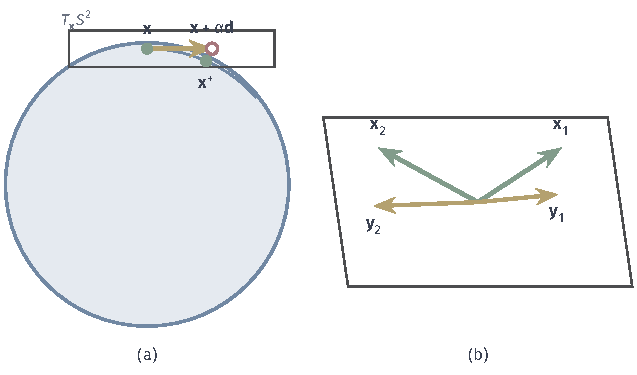
\includegraphics[width=107.9mm]{figures/05-optimization/06-constrained-optimization/tikz/mfo-step-leaves/figure.pdf}
 \caption{欧氏更新破坏光滑约束。(a)~浅蓝球面是可行集，方框是切平面的一块，黄箭头是切向的一步，红圈是落在球面外的点，虚线把它沿径向拉回到绿点。(b)~矩阵$\bm{X}$的两列$\bm{x}_1,\bm{x}_2$（绿）标准正交，方框是它们张成的平面；走一步后的两列$\bm{y}_1,\bm{y}_2$（黄）长度约为$1.094$和$1.144$，内积约为$0.247$，都离开了约束。}
 \label{fig:mfo-step-leaves}
\end{BookInlineFigure}

球面和正交矩阵的集合比一般的弯曲约束多一项便利：它们是光滑流形，而且切空间和回到集合上的运算都有便宜的公式。这一章的问题是：能否把这个集合本身当作计算空间，让迭代从头到尾都在集合上走，同时保留梯度法、Newton法、拟Newton法和信赖域的思路？

路线分三层。第~\ref{sec:mfo-problems}节和第~\ref{sec:mfo-optimality}节确定问题的形式和最优性条件，并算出切向梯度与切向曲率。第~\ref{sec:mfo-operations}节回答迭代缺少的三种运算：走完怎样回到集合上，怎样评价候选步，不同点处的向量怎样比较。

第~\ref{sec:mfo-first-order}节到第~\ref{sec:mfo-trust-region}节依次把这些运算装进一阶方法、二阶方法、拟Newton法和信赖域，每种方法都在上面的小例子上手算几步。第~\ref{sec:mfo-representation}节用子空间问题说明表示方式的影响，并在同一目标和同一精度下比较流形方法与一般约束方法。

\section{流形上的优化问题}
\label{sec:mfo-problems}

什么样的约束集合可以当作计算空间？本节先看两个具体约束，指出它们共有的结构，再说明这一结构在哪些集合上不存在。

\paragraph{两个具体约束}
球面约束$\bm{x}^\top\bm{x}=1$只有一个方程。从点$\bm{x}$出发沿曲线$\bm{c}(t)$运动，并一直留在球面上，就要求$\bm{c}(t)^\top\bm{c}(t)=1$。对$t$求导并取$t=0$，得到速度$\bm{v}=\bm{c}'(0)$必须满足
\[
 \bm{x}^\top\bm{v}=0.
\]
因此$\bm{x}$处允许的运动方向是与$\bm{x}$垂直的全体向量，构成一个$n-1$维的线性子空间。

矩阵约束$\bm{X}^\top\bm{X}=\bm{I}_k$的方程更多。这里$\bm{X}\in\mathbb{R}^{n\times k}$，$k\leq n$，它的列是一组标准正交向量。同样沿曲线$\bm{C}(t)$求导，速度$\bm{\Delta}=\bm{C}'(0)$必须满足
\[
 \bm{X}^\top\bm{\Delta}+\bm{\Delta}^\top\bm{X}=\bm{0}.
\]
这个条件说的是$\bm{X}^\top\bm{\Delta}$是反对称矩阵。例如$n=3$，$k=2$时，矩阵有$6$个元素，约束有$3$个独立方程，所以允许的方向构成一个$3$维子空间。

两个例子的共同点是：约束对变量的允许变化作出限制，而这个限制在每一点都是一个线性子空间，维数处处相同。这正是后面所有方法的立足点，在每一点都有一张平坦的“工作台”，可以在上面做线性代数。

\paragraph{正则等式约束给出流形}
把上面的观察写成一般形式。设$h:\mathbb{R}^n\to\mathbb{R}^p$光滑，可行集是它的零点集：
\begin{equation}
 M=\{\bm{x}\in\mathbb{R}^n:\ h(\bm{x})=\bm{0}\}.
 \label{eq:mfo-level-set}
\end{equation}
记$\bm{J}(\bm{x})$为$h$在$\bm{x}$处的Jacobian矩阵，假定它在$M$的每一点都行满秩。这就是第~\ref{chap:constrained-optimality}章的线性无关约束规范，这里要求它在整个可行集上成立。

这个条件保证$M$是$n-p$维的嵌入子流形，切空间就是Jacobian的零空间：
\begin{equation}
 T_{\bm{x}}M=\ker\bm{J}(\bm{x}).
 \label{eq:mfo-tangent}
\end{equation}
这里用到的是正则水平集定理及切空间的刻画，可参考\BookChapterRef{chap:manifold-relations}{卷四第26章“流形之间的关系”}。球面取$h(\bm{x})=\bm{x}^\top\bm{x}-1$，$\bm{J}(\bm{x})=2\bm{x}^\top$在球面上不为零；矩阵约束取值于对称矩阵，同样满足这个条件。

流形上的优化问题写作
\begin{equation}
 \min_{\bm{x}\in M}\ f(\bm{x}),
 \label{eq:mfo-problem}
\end{equation}
其中$f$定义在包含$M$的开集上并且光滑。本章把$M$就当作前面各章的可行集$\bm{C}$，并沿用卷四的写法把流形记成$M$，把球面记成$S^{n-1}$，把正交列矩阵的集合记成Stiefel流形$\mathrm{St}(k,n)$。问题本身仍是约束极值，改变的只是求解时使用的计算空间。

\paragraph{集合、度量与表示}
“在流形上计算”牵涉三个不同的选择，混淆它们会带来错误的结论。集合$M$由问题决定，它规定了哪些点可行，哪些点是极小点。

\term{黎曼度量}（Riemannian metric）是在每个切空间放一个内积，记为$\langle\bm{u},\bm{v}\rangle_{\bm{x}}$。同一个集合可以配不同的度量。度量决定长度和角度，因而决定“最陡”的方向，但不改变极小点的位置。本章除特别说明外，都取欧氏内积限制到切空间上的诱导度量。

表示方式是在计算机里怎样存一个点。球面上的点可以存成三个坐标，也可以存成两个角度；一个子空间可以存成任意一组基，这时同一个对象有许多矩阵记录。表示决定存储和运算的代价，第~\ref{sec:mfo-representation}节专门讨论。表~\ref{tab:mfo-three-choices}把三者并列。

\begin{BookInlineTable}
 \centering
 \caption{流形优化中三种不同的选择。}
 \label{tab:mfo-three-choices}
 \begin{tabular}{lll}
  \toprule
  选择 & 决定什么 & 不决定什么\\
  \midrule
  集合$M$ & 可行点、极小点 & 梯度的数值\\
  度量$\langle\cdot,\cdot\rangle_{\bm{x}}$ & 梯度、Hessian、步长的尺度 & 极小点的位置\\
  表示 & 存储和运算成本 & 所求的几何对象\\
  \bottomrule
 \end{tabular}
\end{BookInlineTable}

\paragraph{带奇点或棱角的集合}
前面的立足点并非总存在。图~\ref{fig:mfo-regular-singular}对比了三种集合。圆周上每点都有一条切线，法向量$\nabla h$不为零，这是正则的情形。

\begin{BookInlineFigure}
 \centering
 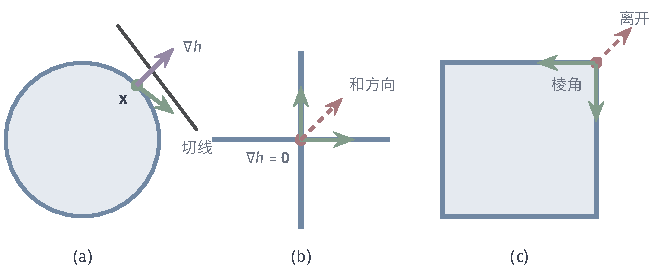
\includegraphics[width=111.9mm]{figures/05-optimization/06-constrained-optimization/tikz/mfo-regular-singular/figure.pdf}
 \caption{三种约束集合。(a)~圆周处处正则，切方向（绿）构成一条直线，紫箭头是约束的梯度。(b)~十字形$x_1x_2=0$在原点处约束梯度为零，两个绿色可行方向之和（红虚线）不可行，可行方向不构成线性子空间。(c)~正方形的角点处，可行方向只有一个锥，朝外的方向（红虚线）不可行。}
 \label{fig:mfo-regular-singular}
\end{BookInlineFigure}

十字形$\{x_1x_2=0\}$在原点处有两条可行的直线，把两个可行方向相加却得到不可行的方向，所以那里没有一个线性的切空间。这里$\nabla(x_1x_2)$在原点为零，正则条件不成立。

棱角的情形类似。方形可行域的角点处，允许的方向只构成一个锥，负向不再允许。这类可行集要用第~\ref{chap:feasible-iterations}章的投影或第~\ref{chap:penalty-multiplier-methods}章的乘子方法，本章的迭代不能直接套用，因为后面每一步都假定当前点处有一个完整的线性切空间。

\section{最优性与导数计算}
\label{sec:mfo-optimality}

普通的判据$\nabla f=\bm{0}$在球面上失效：在极小点$\bm{e}_1$处，$\nabla f$等于$\bm{e}_1$，并不为零。约束下应该把哪个量算成零，怎样判别二阶情形，这些量在具体约束上怎样计算？

\paragraph{切向梯度}
黎曼度量的作用之一是把微分变成向量：$\operatorname{grad}f(\bm{x})$是$T_{\bm{x}}M$中满足下式的唯一向量，$\mathrm{d}f_{\bm{x}}$是$f$在$\bm{x}$处的微分。
\begin{equation}
 \langle\operatorname{grad}f(\bm{x}),\bm{v}\rangle_{\bm{x}}=\mathrm{d}f_{\bm{x}}[\bm{v}],
 \qquad\forall\,\bm{v}\in T_{\bm{x}}M.
 \label{eq:mfo-riem-grad-def}
\end{equation}
这个向量称为\term{黎曼梯度}（Riemannian gradient）。微分和度量的具体定义见\BookChapterRef{chap:manifold-calculus}{卷四第28章“流形上的微积分”}，这里只用它的计算结果。

度量如何影响梯度？设切空间上的内积由对称正定矩阵$\bm{G}$给出，微分的系数向量记为$\bm{c}$。式~\eqref{eq:mfo-riem-grad-def}化成
\[
 \bm{v}^\top\bm{G}\operatorname{grad}f=\bm{v}^\top\bm{c},\qquad\forall\,\bm{v},
\]
于是
\[
 \operatorname{grad}f=\bm{G}^{-1}\bm{c}.
\]
取$\bm{c}=(1,1)^\top$做比较。$\bm{G}=\bm{I}$时梯度是$(1,1)^\top$；$\bm{G}=\operatorname{diag}(4,1)$时梯度是$(\tfrac14,1)^\top$。

图~\ref{fig:mfo-metric-gradient}解释这个差别。绿色区域是该度量下的单位球，梯度方向指向单位球上使线性函数最大的那一点。度量把单位球压扁，切点就移动了。两种度量下，梯度为零的条件都是$\bm{c}=\bm{0}$，所以驻点不受影响。

\begin{BookInlineFigure}
 \centering
 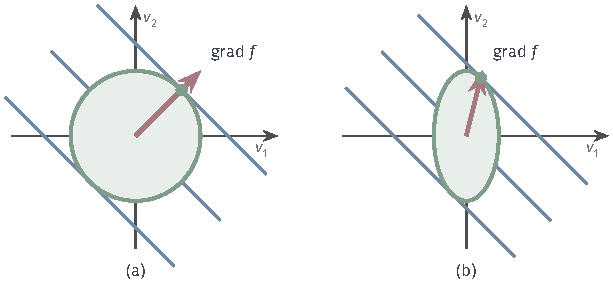
\includegraphics[width=103.8mm]{figures/05-optimization/06-constrained-optimization/tikz/mfo-metric-gradient/figure.pdf}
 \caption{同一微分在两种度量下的梯度。蓝线是线性函数$\mathrm{d}f[\bm{v}]=v_1+v_2$的等值线，绿色区域是度量的单位球，绿点是单位球上函数值最大的点，红箭头是梯度。(a)~$\bm{G}=\bm{I}$。(b)~$\bm{G}=\operatorname{diag}(4,1)$，单位球沿$v_1$被压缩，梯度偏向$v_2$。}
 \label{fig:mfo-metric-gradient}
\end{BookInlineFigure}

\paragraph{诱导度量下用投影计算}
取诱导度量时，黎曼梯度有一个直接的算法。设$\bar{f}$是$f$在环境空间中的光滑延拓，$\bm{P}_{\bm{x}}$是到$T_{\bm{x}}M$的正交投影。下面的引理说明，只要把欧氏梯度投影一下。

\begin{lemma}[投影公式]
 \label{lem:mfo-projection-gradient}
 设$M\subseteq\mathbb{R}^n$是嵌入子流形，取诱导度量，$\bar{f}$在$M$的邻域内光滑且在$M$上等于$f$。则
 \begin{equation}
  \operatorname{grad}f(\bm{x})=\bm{P}_{\bm{x}}\nabla\bar{f}(\bm{x}).
  \label{eq:mfo-projection-gradient}
 \end{equation}
\end{lemma}

\begin{proof}
 对$\bm{v}\in T_{\bm{x}}M$，取$M$上的曲线$\bm{c}$，满足$\bm{c}(0)=\bm{x}$，$\bm{c}'(0)=\bm{v}$。因为$f$与$\bar{f}$在$M$上相等，
 \[
  \mathrm{d}f_{\bm{x}}[\bm{v}]=\frac{\mathrm{d}}{\mathrm{d}t}\bar{f}(\bm{c}(t))\Big|_{t=0}=\langle\nabla\bar{f}(\bm{x}),\bm{v}\rangle.
 \]

 $\bm{P}_{\bm{x}}$是正交投影，$\bm{v}$在切空间中，所以$\bm{P}_{\bm{x}}\bm{v}=\bm{v}$，并且投影对称，于是
 \[
  \langle\nabla\bar{f}(\bm{x}),\bm{v}\rangle=\langle\nabla\bar{f}(\bm{x}),\bm{P}_{\bm{x}}\bm{v}\rangle=\langle\bm{P}_{\bm{x}}\nabla\bar{f}(\bm{x}),\bm{v}\rangle.
 \]
 $\bm{P}_{\bm{x}}\nabla\bar{f}(\bm{x})$在切空间中，又满足定义式~\eqref{eq:mfo-riem-grad-def}，由唯一性得结论。
\end{proof}

投影公式的适用条件是诱导度量，这一点不能省略。换了别的度量，还须按上一段的公式乘以度量的逆。

\paragraph{球面Rayleigh商}
把公式用到贯穿例。球面上的投影去掉沿$\bm{x}$的分量：
\[
 \bm{P}_{\bm{x}}\bm{z}=\bm{z}-(\bm{x}^\top\bm{z})\bm{x}.
\]

记\term{Rayleigh商}（Rayleigh quotient）的取值为$q(\bm{x})=\bm{x}^\top\bm{A}\bm{x}$，这里$\lVert\bm{x}\rVert_2=1$。欧氏梯度是$\bm{A}\bm{x}$，$\bm{x}^\top\bm{A}\bm{x}=q$，所以
\begin{equation}
 \operatorname{grad}f(\bm{x})=\bm{A}\bm{x}-q(\bm{x})\bm{x}.
 \label{eq:mfo-rayleigh-grad}
\end{equation}

在起点$\bm{x}^{(0)}$上算一遍。先算下面三个量：
\[
 \bm{A}\bm{x}^{(0)}=\frac13(2,4,4)^\top,\qquad q(\bm{x}^{(0)})=\frac{4+8+4}{9}=\frac{16}{9}.
\]
代入式~\eqref{eq:mfo-rayleigh-grad}，得到
\[
 \bm{g}^{(0)}=\frac13(2,4,4)^\top-\frac{16}{27}(2,2,1)^\top=\frac{1}{27}(-14,4,20)^\top.
\]

可以检查它在切空间中：$\bm{x}^{(0)\top}\bm{g}^{(0)}=(-28+8+20)/81=0$。范数的平方是
\[
 \lVert\bm{g}^{(0)}\rVert_2^2=\frac{196+16+400}{729}=\frac{68}{81}.
\]

图~\ref{fig:mfo-tangent-projection}画出这次分解。蓝色的欧氏梯度分成两段，紫色部分沿法向，只会改变到球面的距离，绿色部分才对球面上的运动起作用。

\begin{BookInlineFigure}
 \centering
 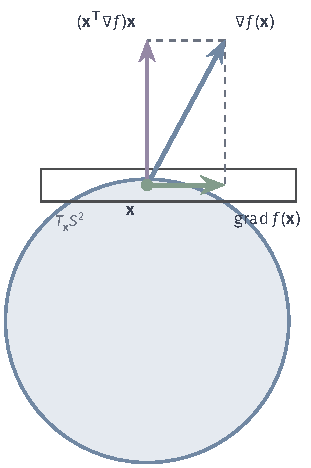
\includegraphics[width=52.7mm]{figures/05-optimization/06-constrained-optimization/tikz/mfo-tangent-projection/figure.pdf}
 \caption{起点$\bm{x}^{(0)}$处欧氏梯度的分解。蓝箭头是$\nabla f$，紫箭头是法向分量，绿箭头是切向分量即黎曼梯度，方框是切平面的一块。三个箭头按同一比例缩短到原长的$0.6$倍。}
 \label{fig:mfo-tangent-projection}
\end{BookInlineFigure}

\paragraph{一阶条件与Lagrange乘子}
现在把切向梯度与第~\ref{chap:constrained-optimality}章的乘子联系起来。由式~\eqref{eq:mfo-tangent}，$T_{\bm{x}}M$的正交投影可以写成
\[
 \bm{P}_{\bm{x}}=\bm{I}-\bm{J}^\top(\bm{J}\bm{J}^\top)^{-1}\bm{J},
\]
这里行满秩保证$\bm{J}\bm{J}^\top$可逆。

把投影代入式~\eqref{eq:mfo-projection-gradient}，并定义乘子
\begin{equation}
 \bm{\nu}(\bm{x})=-(\bm{J}\bm{J}^\top)^{-1}\bm{J}\nabla\bar{f}(\bm{x}),
 \label{eq:mfo-ls-multiplier}
\end{equation}
就得到
\begin{equation}
 \operatorname{grad}f(\bm{x})=\nabla\bar{f}(\bm{x})+\bm{J}(\bm{x})^\top\bm{\nu}(\bm{x})=\nabla_{\bm{x}}\mathcal{L}(\bm{x},\bm{\nu}(\bm{x})).
 \label{eq:mfo-grad-lagrange}
\end{equation}
所以黎曼梯度正是Lagrange函数对$\bm{x}$的梯度，乘子取使$\lVert\nabla\bar{f}+\bm{J}^\top\bm{\nu}\rVert_2$最小的最小二乘乘子。黎曼梯度为零，就是Lagrange乘子驻定条件。

球面上$h(\bm{x})=\bm{x}^\top\bm{x}-1$，$\bm{J}=2\bm{x}^\top$，$\bm{J}\bm{J}^\top=4$，代入式~\eqref{eq:mfo-ls-multiplier}得到
\[
 \nu(\bm{x})=-\frac14\cdot2\bm{x}^\top\bm{A}\bm{x}=-\frac12q(\bm{x}).
\]
梯度为零的条件$\bm{A}\bm{x}=q\bm{x}$说明，驻点恰好是$\bm{A}$的单位特征向量，并且$q$就是特征值。贯穿例有六个驻点$\pm\bm{e}_1,\pm\bm{e}_2,\pm\bm{e}_3$。

图~\ref{fig:mfo-rayleigh-landscape}是目标在球面上的等高线。红点$\bm{e}_1$周围的闭合曲线表明这里是极小点，$\bm{e}_3$是极大点，$\bm{e}_2$处等高线呈交叉状，它是鞍点。

\begin{BookInlineFigure}
 \centering
 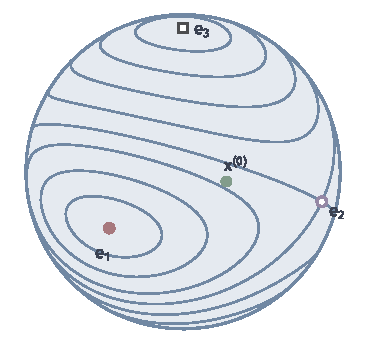
\includegraphics[width=62.0mm]{figures/05-optimization/06-constrained-optimization/matplotlib/mfo-rayleigh-landscape/figure.pdf}
 \caption{贯穿例的目标在单位球面上的等高线（蓝），只画朝向读者的半球。红点是极小点$\bm{e}_1$，紫圈是鞍点$\bm{e}_2$，方块是极大点$\bm{e}_3$，绿点是起点。背面半球的$-\bm{e}_1,-\bm{e}_2,-\bm{e}_3$有相同的情形。}
 \label{fig:mfo-rayleigh-landscape}
\end{BookInlineFigure}

\paragraph{切向曲率}
一阶条件分不开$\bm{e}_1,\bm{e}_2,\bm{e}_3$，需要二阶信息。\term{黎曼Hessian}（Riemannian Hessian）是切空间$T_{\bm{x}}M$到自身的对称线性算子，记为$\operatorname{Hess}f(\bm{x})$，定义为黎曼梯度沿切向量的协变导数，其几何来历可参考\BookChapterRef{chap:riemannian-geometry}{卷四第27章“黎曼几何”}。

诱导度量下的协变导数是先做普通方向导数再投影，所以只要把黎曼梯度光滑延拓成环境空间中的向量场$\bm{G}$，就有
\begin{equation}
 \operatorname{Hess}f(\bm{x})[\bm{v}]=\bm{P}_{\bm{x}}\,\mathrm{D}\bm{G}(\bm{x})[\bm{v}].
 \label{eq:mfo-hess-projection}
\end{equation}

球面上把式~\eqref{eq:mfo-rayleigh-grad}的右端在整个空间中当作$\bm{G}(\bm{x})$，方向导数是
\[
 \mathrm{D}\bm{G}(\bm{x})[\bm{v}]=\bm{A}\bm{v}-2(\bm{x}^\top\bm{A}\bm{v})\bm{x}-q(\bm{x})\bm{v}.
\]
第二项沿法向，投影后消失；第三项本身是切向的。于是
\begin{equation}
 \operatorname{Hess}f(\bm{x})[\bm{v}]=\bm{P}_{\bm{x}}\bigl(\bm{A}\bm{v}\bigr)-q(\bm{x})\bm{v},\qquad \bm{v}\perp\bm{x}.
 \label{eq:mfo-rayleigh-hess}
\end{equation}

这个式子里的$-q\bm{v}$值得留意。欧氏Hessian是$\bm{A}$，而切向曲率还要减去$q$，这一项来自约束本身的弯曲，由乘子项承担，下面马上看到。

在驻点上用这个公式。取$\bm{x}=\bm{e}_i$，$q=\lambda_i$，切空间由其余两个坐标向量张成，算子是对角的。三个驻点的切向曲率如表~\ref{tab:mfo-critical}所示。

\begin{BookInlineTable}
 \centering
 \caption{贯穿例的驻点，切向曲率由式~\eqref{eq:mfo-rayleigh-hess}算出。}
 \label{tab:mfo-critical}
 \begin{tabular}{llll}
  \toprule
  驻点 & $q$ & 切向曲率 & 类型\\
  \midrule
  $\pm\bm{e}_1$ & $1$ & $2-1=1,\ 4-1=3$ & 严格局部极小，全局极小\\
  $\pm\bm{e}_2$ & $2$ & $1-2=-1,\ 4-2=2$ & 鞍点\\
  $\pm\bm{e}_3$ & $4$ & $1-4=-3,\ 2-4=-2$ & 严格局部极大\\
  \bottomrule
 \end{tabular}
\end{BookInlineTable}

图~\ref{fig:mfo-critical-local}把三类驻点放到各自的切平面坐标里看。图中的函数值是把切向量先归一化回球面后计算的，局部形状与表中的符号一致。

\begin{BookInlineFigure}
 \centering
 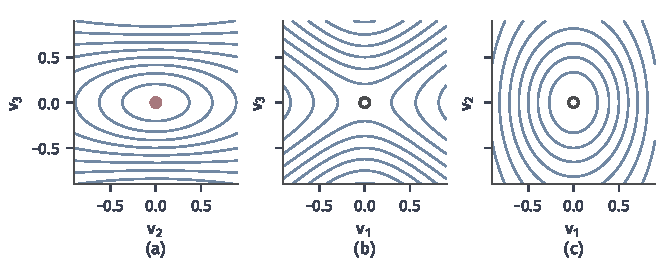
\includegraphics[width=112.0mm]{figures/05-optimization/06-constrained-optimization/matplotlib/mfo-critical-local/figure.pdf}
 \caption{三类驻点附近的局部形状。蓝线是$f(\bm{x}+\bm{v})/\lVert\bm{x}+\bm{v}\rVert_2^2$的等值线，这里的$f$在贯穿例中是二次齐次的，该式等于把$\bm{x}+\bm{v}$归一化后的目标值。$(v_i,v_j)$是切平面坐标。(a)~$\bm{e}_1$，碗形。(b)~$\bm{e}_2$，马鞍形。(c)~$\bm{e}_3$，倒扣的碗。}
 \label{fig:mfo-critical-local}
\end{BookInlineFigure}

\paragraph{曲率与Lagrange函数的Hessian}
为什么约束的弯曲会以乘子的形式进入？设$\bm{c}(t)$是$M$上的曲线，$\bm{c}(0)=\bm{x}$，$\bm{c}'(0)=\bm{v}$。由$h_j(\bm{c}(t))=0$求两次导，得到
\[
 \nabla h_j(\bm{x})^\top\bm{c}''(0)+\bm{v}^\top\nabla^2h_j(\bm{x})\bm{v}=0.
\]

现在求目标沿曲线的二阶导数，它是
\[
 (\bar{f}\circ\bm{c})''(0)=\bm{v}^\top\nabla^2\bar{f}\bm{v}+\nabla\bar{f}^\top\bm{c}''(0).
\]
由式~\eqref{eq:mfo-grad-lagrange}把$\nabla\bar{f}$换成黎曼梯度减去$\bm{J}^\top\bm{\nu}$，再利用上一式把$\nabla h_j^\top\bm{c}''(0)$换掉，就得到
\begin{equation}
 (\bar{f}\circ\bm{c})''(0)=\bm{v}^\top\nabla^2_{\bm{x}\bm{x}}\mathcal{L}(\bm{x},\bm{\nu}(\bm{x}))\bm{v}+\bigl\langle\operatorname{grad}f(\bm{x}),\bm{c}''(0)\bigr\rangle.
 \label{eq:mfo-second-along-curve}
\end{equation}

测地线的加速度是纯法向的，所以取$\bm{c}$为测地线时最后一项为零，左端就是$\langle\bm{v},\operatorname{Hess}f(\bm{x})[\bm{v}]\rangle$。这样切向曲率等于Lagrange函数的Hessian在切空间上的二次型：
\begin{equation}
 \langle\bm{v},\operatorname{Hess}f(\bm{x})[\bm{v}]\rangle=\bm{v}^\top\nabla^2_{\bm{x}\bm{x}}\mathcal{L}(\bm{x},\bm{\nu}(\bm{x}))\bm{v},\qquad\bm{v}\in T_{\bm{x}}M.
 \label{eq:mfo-hess-lagrange}
\end{equation}

球面上核对一下。Lagrange函数的Hessian是
\[
 \nabla^2_{\bm{x}\bm{x}}\mathcal{L}=\bm{A}+2\nu\bm{I}=\bm{A}-q\bm{I},
\]
所以二次型是$\bm{v}^\top\bm{A}\bm{v}-q\lVert\bm{v}\rVert_2^2$，与式~\eqref{eq:mfo-rayleigh-hess}相同。式~\eqref{eq:mfo-second-along-curve}最后那一项在第~\ref{sec:mfo-pullback}节还会用到。

\paragraph{二阶判别}
下面的定理把上述量组织成判别条件，要分清必要与充分。

\begin{theorem}[流形上的最优性条件]
 \label{thm:mfo-optimality}
 设$f$在黎曼流形$M$上二阶连续可微，$\bm{x}^\star\in M$。
 \begin{enumerate}
  \item 若$\bm{x}^\star$是局部极小点，则$\operatorname{grad}f(\bm{x}^\star)=\bm{0}$，且$\operatorname{Hess}f(\bm{x}^\star)$半正定。
  \item 若$\operatorname{grad}f(\bm{x}^\star)=\bm{0}$，且$\operatorname{Hess}f(\bm{x}^\star)$在$T_{\bm{x}^\star}M$上正定，则$\bm{x}^\star$是严格局部极小点。
 \end{enumerate}
\end{theorem}

\begin{proof}
 记指数映射为$\exp_{\bm{x}^\star}$，定义切空间上的函数
 \[
  \phi(\bm{v})=f(\exp_{\bm{x}^\star}(\bm{v})).
 \]

 指数映射在零点的微分是恒等映射，由反函数定理，它把零点的一个邻域微分同胚地映到$\bm{x}^\star$的一个邻域。

 因此$\bm{x}^\star$是$f$的（严格）局部极小点，当且仅当$\bm{0}$是$\phi$的（严格）局部极小点。对单位切向量$\bm{v}$，曲线$\gamma(t)=\exp_{\bm{x}^\star}(t\bm{v})$是测地线，于是
 \[
  \frac{\mathrm{d}}{\mathrm{d}t}\phi(t\bm{v})\Big|_{t=0}=\langle\operatorname{grad}f(\bm{x}^\star),\bm{v}\rangle,
  \qquad
  \frac{\mathrm{d}^2}{\mathrm{d}t^2}\phi(t\bm{v})\Big|_{t=0}=\langle\bm{v},\operatorname{Hess}f(\bm{x}^\star)[\bm{v}]\rangle.
 \]
 这说明$\phi$在零点的欧氏梯度和Hessian正是黎曼梯度和黎曼Hessian。把线性空间上无约束问题的一阶、二阶必要条件和二阶充分条件用到$\phi$上，就得到两个结论。
\end{proof}

两个条件之间有间隙，$\operatorname{Hess}f$半正定但不正定时，定理不作结论。取圆周上的$f(\bm{x})=x_2^3$，在点$(1,0)$处切向坐标为$\theta$，$f=\sin^3\theta$的一阶、二阶导数都为零，二阶必要条件成立，但$\theta<0$时函数值更小，这一点不是局部极小。

半正定也可能来自一整段极小点。取$\bm{A}=\operatorname{diag}(1,1,4)$，圆周$x_3=0$上每一点都是全局极小点，切向曲率有一个零方向，定理第二条不适用，这些点并不是孤立的。

定理也只是局部结论。圆周上的$\cos3\theta+0.3\cos\theta$在$\theta=\pi$附近和$\theta=\pm\pi/3$附近都有严格局部极小，函数值分别约为$-1.30$和$-0.85$，后者满足二阶充分条件却不是全局极小。

Rayleigh商是一个少见的例外，局部极小都是全局极小。设$\bm{x}$是特征向量，特征值$\lambda>\lambda_1$，取$\lambda_1$的单位特征向量$\bm{v}$，它与$\bm{x}$正交，由式~\eqref{eq:mfo-rayleigh-hess}得到
\[
 \langle\bm{v},\operatorname{Hess}f(\bm{x})[\bm{v}]\rangle=\lambda_1-\lambda<0.
\]
所以满足二阶必要条件的驻点只能属于最小特征值。这个结论来自目标的特殊结构，不能推广到一般流形问题。

\section{迭代的几何运算}
\label{sec:mfo-operations}

现在假定当前点$\bm{x}$处已经算出一个切向候选步$\bm{v}\in T_{\bm{x}}M$。欧氏空间里接下来的事情都是加减法，到了流形上有三件事要重新回答：走完之后怎样回到集合上，怎样评价这一步好不好，历史上的向量在新点怎样使用。

图~\ref{fig:mfo-iteration-loop}是后面所有算法共用的循环。切向候选步由各节的方法给出，其余三个方框分别由下面三小节回答。这里只讨论能在计算机上执行的运算，切空间、联络和指数映射的定义仍以卷四为准。

\begin{BookInlineFigure}
 \centering
 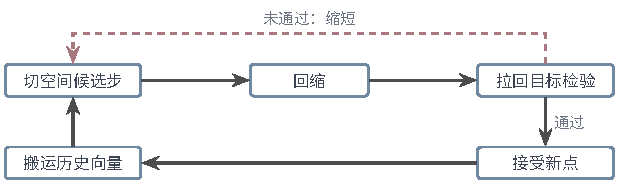
\includegraphics[width=104.7mm]{figures/05-optimization/06-constrained-optimization/tikz/mfo-iteration-loop/figure.pdf}
 \caption{流形优化的一轮迭代。切空间里产生候选步，回缩把它变成流形上的候选点，再用拉回后的目标判断是否接受；接受后把需要保留的历史向量搬到新点的切空间。红色虚线表示判断未通过时缩短步长或半径。}
 \label{fig:mfo-iteration-loop}
\end{BookInlineFigure}

\subsection{回缩}
\label{sec:mfo-retraction}

\paragraph{用球面看需要什么}
从$\bm{x}$走到$\bm{x}+\bm{v}$后，最自然的修正是除以长度，把点拉回球面：
\begin{equation}
 R_{\bm{x}}(\bm{v})=\frac{\bm{x}+\bm{v}}{\lVert\bm{x}+\bm{v}\rVert_2}=\frac{\bm{x}+\bm{v}}{\sqrt{1+\lVert\bm{v}\rVert_2^2}}.
 \label{eq:mfo-sphere-retraction}
\end{equation}
第二个等号用到$\bm{x}\perp\bm{v}$和勾股定理。这个映射有两条关键性质：零步不动，并且走很小的一步时，它和切向量给出的方向一致。

把第二条写成曲线的语言。令$\bm{c}(t)=R_{\bm{x}}(t\bm{v})$，把分母按$t$展开，得到
\[
 \bm{c}(t)=(\bm{x}+t\bm{v})\Bigl(1-\frac12t^2\lVert\bm{v}\rVert_2^2+O(t^4)\Bigr).
\]
由此读出$\bm{c}(0)=\bm{x}$，$\bm{c}'(0)=\bm{v}$，加速度$\bm{c}''(0)=-\lVert\bm{v}\rVert_2^2\bm{x}$沿法向。

这两条性质正是我们真正需要的，再多的要求（例如走出的曲线恰好是测地线）对一阶信息没有帮助。于是有下面的定义。

\begin{definition}[回缩]
 \label{def:mfo-retraction}
 流形$M$上的\term{回缩}（retraction）是一族光滑映射$R_{\bm{x}}:U_{\bm{x}}\to M$，其中$U_{\bm{x}}$是$T_{\bm{x}}M$中包含零的开集，并且对所有$\bm{x}\in M$，$\bm{v}\in T_{\bm{x}}M$有
 \begin{equation}
  R_{\bm{x}}(\bm{0})=\bm{x},\qquad
  \frac{\mathrm{d}}{\mathrm{d}t}R_{\bm{x}}(t\bm{v})\Big|_{t=0}=\bm{v}.
  \label{eq:mfo-retraction-def}
 \end{equation}
 若进一步对所有$\bm{v}$，曲线$\bm{c}(t)=R_{\bm{x}}(t\bm{v})$的加速度满足$\bm{P}_{\bm{x}}\bm{c}''(0)=\bm{0}$，则称它为\term{二阶回缩}（second-order retraction）。
\end{definition}

二阶条件的提法依赖诱导度量：对嵌入子流形，它说的是加速度的切向分量为零。指数映射是最典型的二阶回缩，因为测地线加速度的切向分量恒为零。式~\eqref{eq:mfo-sphere-retraction}由上面的展开也是二阶回缩。

\paragraph{回缩不等于指数映射}
图~\ref{fig:mfo-retraction-cut}(a)在穿过球心的截面上比较两种走法。切向量长度为$s$时，指数映射沿大圆走过角度$s$，归一化走过角度$\arctan s$。

\begin{BookInlineFigure}
 \centering
 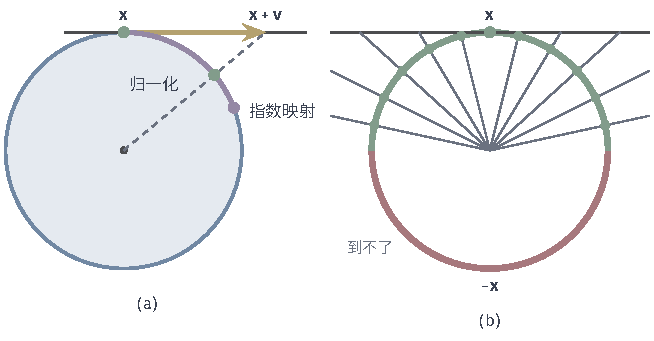
\includegraphics[width=110.8mm]{figures/05-optimization/06-constrained-optimization/tikz/mfo-retraction-cut/figure.pdf}
 \caption{球面的截面。(a)~黄箭头是长度$1.2$的切向量，归一化把它的端点沿虚线径向拉回到绿点，紫弧是指数映射走过的路，端点在紫点。(b)~切线上的点全都被归一化映到上半圆（绿）。下半圆（红）到不了，对跖点$-\bm{x}$也到不了。}
 \label{fig:mfo-retraction-cut}
\end{BookInlineFigure}

两者的差在小步时很小。由$\arctan s=s-s^3/3+O(s^5)$，角度差是$s^3/3$的量级，这是图~\ref{fig:mfo-retraction-error}(b)的斜率$3$。步子大了差距才明显：$s\to\infty$时归一化只能逼近$\pi/2$，而指数映射走过的角度不断增长。

\begin{BookInlineFigure}
 \centering
 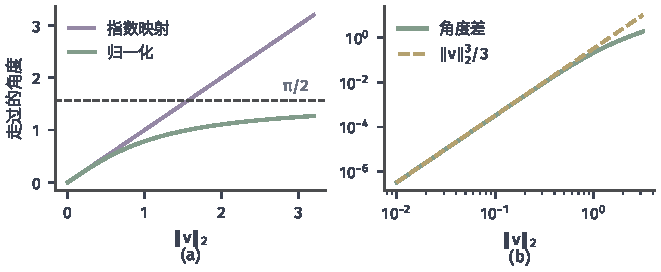
\includegraphics[width=112.0mm]{figures/05-optimization/06-constrained-optimization/matplotlib/mfo-retraction-error/figure.pdf}
 \caption{球面上切向量长度$\lVert\bm{v}\rVert_2$与走过的角度。(a)~指数映射（紫）的角度等于长度，归一化（绿）的角度不超过$\pi/2$。(b)~双对数坐标下两者的角度差（绿）与$\lVert\bm{v}\rVert_2^3/3$（黄虚线）在小步时重合。}
 \label{fig:mfo-retraction-error}
\end{BookInlineFigure}

把切平面整张折到球面上，就看到回缩的全貌。图~\ref{fig:mfo-retraction-grid}中，切平面上等间距的同心圆经过归一化后向边缘挤压，径向的射线变成大圆。这也提醒我们，回缩不是等距的，切空间里的长度只在原点附近才代表流形上走过的距离。

\begin{BookInlineFigure}
 \centering
 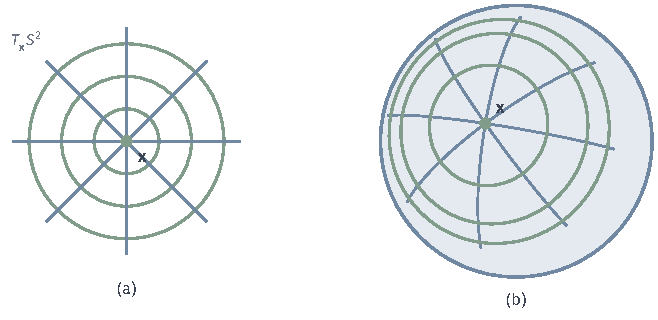
\includegraphics[width=111.3mm]{figures/05-optimization/06-constrained-optimization/tikz/mfo-retraction-grid/figure.pdf}
 \caption{归一化回缩把切平面折到球面上。(a)~切平面上半径$0.5,1,1.5$的同心圆（绿）与八条射线（蓝）。(b)~它们在回缩下的像，同心圆的间距向外收紧，射线变成大圆的一段。}
 \label{fig:mfo-retraction-grid}
\end{BookInlineFigure}

\paragraph{定义域}
归一化公式对所有切向量都有定义，因为$\bm{x}\perp\bm{v}$保证$\bm{x}+\bm{v}\neq\bm{0}$，但它的像只覆盖开上半球，如图~\ref{fig:mfo-retraction-cut}(b)所示。定义~\ref{def:mfo-retraction}只要求在零的邻域内有定义，这对迭代是足够的，因为每步只需要局部信息。

一般回缩可能只在局部有定义，分解还可能有多种选择。选择不固定就会使映射不光滑，下面的矩阵例子就有这个问题。

\paragraph{Stiefel流形上的回缩}
取$\bm{X}\in\mathrm{St}(k,n)$，切向量$\bm{\Delta}$满足$\bm{X}^\top\bm{\Delta}$反对称。把$\bm{X}+\bm{\Delta}$作QR分解$\bm{X}+\bm{\Delta}=\bm{Q}\bm{R}$，其中$\bm{R}$上三角且对角元为正，取$\bm{Q}$作为新点：
\begin{equation}
 R_{\bm{X}}^{\mathrm{QR}}(\bm{\Delta})=\bm{Q}.
 \label{eq:mfo-qr-retraction}
\end{equation}

固定对角元为正这个选择是必要的，否则列的符号可以任意翻转，映射甚至不连续。分解一定存在且唯一，因为$\bm{X}^\top\bm{\Delta}$反对称使两个交叉项抵消：
\[
 (\bm{X}+\bm{\Delta})^\top(\bm{X}+\bm{\Delta})=\bm{I}+\bm{\Delta}^\top\bm{\Delta}\succ\bm{0},
\]
所以$\bm{X}+\bm{\Delta}$列满秩。

下面核对一阶一致性。令$\bm{X}+t\bm{\Delta}=\bm{Q}(t)\bm{R}(t)$，$\bm{Q}(0)=\bm{X}$，$\bm{R}(0)=\bm{I}$。对$t$求导并在$t=0$左乘$\bm{X}^\top$，得到
\[
 \bm{X}^\top\bm{\Delta}=\bm{X}^\top\bm{Q}'(0)+\bm{R}'(0).
\]

左端反对称，右端第一项也反对称（对$\bm{Q}(t)^\top\bm{Q}(t)=\bm{I}$求导得到），所以$\bm{R}'(0)$既反对称又上三角，只能是零。代回求导式就得到$\bm{Q}'(0)=\bm{\Delta}$。

第二种构造用极分解，把$\bm{X}+\bm{\Delta}$的列正交化的同时尽量少动它：
\begin{equation}
 R_{\bm{X}}^{\mathrm{pol}}(\bm{\Delta})=(\bm{X}+\bm{\Delta})\bigl(\bm{I}+\bm{\Delta}^\top\bm{\Delta}\bigr)^{-1/2}.
 \label{eq:mfo-polar-retraction}
\end{equation}

结果确实在流形上：列满秩矩阵右乘$(\bm{Y}^\top\bm{Y})^{-1/2}$后列标准正交。把逆平方根展开，得到
\[
 \bm{C}(t)=(\bm{X}+t\bm{\Delta})\Bigl(\bm{I}-\frac12t^2\bm{\Delta}^\top\bm{\Delta}+O(t^4)\Bigr).
\]
于是$\bm{C}'(0)=\bm{\Delta}$，$\bm{C}''(0)=-\bm{X}\bm{\Delta}^\top\bm{\Delta}$。

后者形如$\bm{X}\bm{B}$，其中$\bm{B}$对称。为了判断它的切向分量，写出$\mathrm{St}(k,n)$的切向投影
\begin{equation}
 \bm{P}_{\bm{X}}(\bm{Z})=\bm{Z}-\bm{X}\operatorname{sym}(\bm{X}^\top\bm{Z}),\qquad \operatorname{sym}(\bm{B})=\frac12(\bm{B}+\bm{B}^\top).
 \label{eq:mfo-stiefel-projection}
\end{equation}
把$\bm{Z}=\bm{X}\bm{B}$代入，得到$\bm{X}\bm{B}-\bm{X}\bm{B}=\bm{0}$，所以极分解回缩是二阶回缩。QR回缩一般只是一阶的，下面的例子中它的加速度有非零的切向分量。

用具体数字比较两种构造。在$\mathrm{St}(2,3)$上取
\[
 \bm{X}=\begin{bmatrix}1&0\\0&1\\0&0\end{bmatrix},\qquad
 \bm{\Delta}=\begin{bmatrix}0&0\\0&0\\1&1\end{bmatrix},\qquad
 \bm{Y}=\bm{X}+\bm{\Delta}=\begin{bmatrix}1&0\\0&1\\1&1\end{bmatrix}.
\]
这里$\bm{X}^\top\bm{\Delta}=\bm{0}$，是切向量。

QR分解按列正交化。第一列除以$\sqrt2$，第二列减去在第一列上的投影再除以长度，于是
\[
 \bm{q}_1=\frac{1}{\sqrt2}(1,0,1)^\top,\qquad
 \bm{q}_2=\frac{1}{\sqrt6}(-1,2,1)^\top.
\]

极分解要用$\bm{I}+\bm{\Delta}^\top\bm{\Delta}$的逆平方根。这个矩阵是
\[
 \bm{I}+\bm{\Delta}^\top\bm{\Delta}=\begin{bmatrix}2&1\\1&2\end{bmatrix},
\]
特征值为$3,1$，特征向量为$(1,1)^\top/\sqrt2$和$(1,-1)^\top/\sqrt2$，算出来的结果是
\[
 R_{\bm{X}}^{\mathrm{pol}}(\bm{\Delta})\approx\begin{bmatrix}0.7887&-0.2113\\-0.2113&0.7887\\0.5774&0.5774\end{bmatrix}.
\]

沿曲线$R_{\bm{X}}(t\bm{\Delta})$算加速度的切向分量，极分解得到零，QR回缩得到
\[
 \bm{P}_{\bm{X}}\bm{C}''(0)=\begin{bmatrix}0&-1\\1&0\\0&0\end{bmatrix},
\]
不是零，这印证了两者阶数的差别。

图~\ref{fig:mfo-stiefel-qr-polar}画出两个结果。QR分解保留第一列的方向，把调整都压给后面的列，极分解则两列对称地调整。两个新点张成同一个平面，这个事实在第~\ref{sec:mfo-representation}节会派上用场。

\begin{BookInlineFigure}
 \centering
 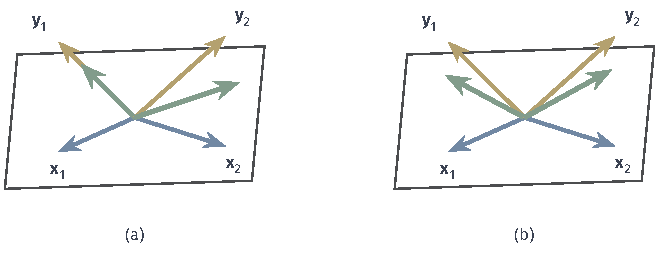
\includegraphics[width=111.6mm]{figures/05-optimization/06-constrained-optimization/tikz/mfo-stiefel-qr-polar/figure.pdf}
 \caption{$\mathrm{St}(2,3)$上的两种回缩。蓝箭头是当前两列，黄箭头是$\bm{X}+\bm{\Delta}$的两列，绿箭头是回缩结果，方框是$\bm{y}_1,\bm{y}_2$张成的平面。(a)~QR分解：第一列方向不变。(b)~极分解：两列对称调整。}
 \label{fig:mfo-stiefel-qr-polar}
\end{BookInlineFigure}

\paragraph{回缩、指数映射与最近点}
第三个候选是把$\bm{x}+\bm{v}$投影到$M$上的最近点。球面上它恰好就是归一化；$\mathrm{St}(k,n)$上在Frobenius范数下恰好就是极分解，例中极分解结果到$\bm{Y}$的距离约为$0.732$，QR结果约为$0.850$。

但回缩并不要求求解最近点问题。QR回缩不是最近点，同样满足定义，而且通常更便宜。在一般曲面上，最近点可能需要迭代才能算出，甚至不唯一。表~\ref{tab:mfo-retraction-compare}比较三者。

\begin{BookInlineTable}
 \centering
 \caption{三种回到流形的方式。“二阶”的结论对最近点投影要求流形足够光滑，表中代价按一次运算计。}
 \label{tab:mfo-retraction-compare}
 \begin{tabular}{llll}
  \toprule
  方式 & 阶 & 球面 & Stiefel\\
  \midrule
  指数映射 & 二阶 & $O(n)$ & 需矩阵指数\\
  最近点投影 & 二阶 & $O(n)$ & 需SVD\\
  QR回缩 & 一阶 & 同归一化 & 约$O(nk^2)$\\
  \bottomrule
 \end{tabular}
\end{BookInlineTable}

\subsection{目标拉回}
\label{sec:mfo-pullback}

\paragraph{把问题搬到同一个切空间}
候选步是切空间中的向量，而目标定义在流形上。把两者复合，就得到切空间上的普通函数，这是后面评价候选步的唯一依据。

\begin{definition}[拉回目标]
 \label{def:mfo-pullback}
 在$\bm{x}\in M$处，目标$f$的\term{拉回}（pullback）是切空间上的函数
 \begin{equation}
  \hat{f}_{\bm{x}}(\bm{v})=f\bigl(R_{\bm{x}}(\bm{v})\bigr),\qquad\bm{v}\in U_{\bm{x}}.
  \label{eq:mfo-pullback}
 \end{equation}
\end{definition}

这个定义的好处是，$\hat{f}_{\bm{x}}$活在线性空间上，前面各章的工具（Taylor展开、Armijo条件、预测下降）都可以直接使用。

贯穿例在$\bm{x}^{(0)}$的切平面上取一组标准正交基：
\[
 \bm{E}_1=\frac13(1,-2,2)^\top,\qquad
 \bm{E}_2=\frac13(2,-1,-2)^\top.
\]
可以检查$\bm{x}^{(0)},\bm{E}_1,\bm{E}_2$两两正交且长度为一。

沿$\bm{v}=s\bm{E}_2$拉回。需要的内积是$\bm{x}^{(0)\top}\bm{A}\bm{E}_2=-\tfrac89$和$\bm{E}_2^\top\bm{A}\bm{E}_2=\tfrac{22}{9}$，代入归一化回缩，得到
\begin{equation}
 \hat{f}_{\bm{x}^{(0)}}(s\bm{E}_2)=\frac{1}{1+s^2}\cdot\frac12\Bigl(\frac{16}{9}-\frac{16}{9}s+\frac{22}{9}s^2\Bigr)=\frac{8-8s+11s^2}{9(1+s^2)}.
 \label{eq:mfo-pullback-line}
\end{equation}

\paragraph{一阶与二阶变化}
下面的引理说明，拉回在零点的一阶信息总是黎曼梯度，二阶信息则取决于回缩的加速度。

\begin{lemma}[拉回的导数]
 \label{lem:mfo-pullback-derivatives}
 设$M$是嵌入子流形，取诱导度量，$R$是回缩，$\bm{v}\in T_{\bm{x}}M$，$\bm{c}(t)=R_{\bm{x}}(t\bm{v})$。则
 \begin{equation}
  \nabla\hat{f}_{\bm{x}}(\bm{0})=\operatorname{grad}f(\bm{x}),
  \label{eq:mfo-pullback-grad}
 \end{equation}
 \begin{equation}
  \langle\bm{v},\nabla^2\hat{f}_{\bm{x}}(\bm{0})\bm{v}\rangle=\langle\bm{v},\operatorname{Hess}f(\bm{x})[\bm{v}]\rangle+\bigl\langle\operatorname{grad}f(\bm{x}),\bm{c}''(0)\bigr\rangle.
  \label{eq:mfo-pullback-hess}
 \end{equation}
\end{lemma}

\begin{proof}
 由复合函数求导和式~\eqref{eq:mfo-retraction-def}，
 \[
  \frac{\mathrm{d}}{\mathrm{d}t}\hat{f}_{\bm{x}}(t\bm{v})\Big|_{t=0}=\mathrm{d}f_{\bm{x}}[\bm{c}'(0)]=\mathrm{d}f_{\bm{x}}[\bm{v}]=\langle\operatorname{grad}f(\bm{x}),\bm{v}\rangle,
 \]
 这是式~\eqref{eq:mfo-pullback-grad}。

 $\hat{f}_{\bm{x}}(t\bm{v})=f(\bm{c}(t))$，把式~\eqref{eq:mfo-second-along-curve}用到曲线$\bm{c}$上，再用式~\eqref{eq:mfo-hess-lagrange}替换第一项，就得到式~\eqref{eq:mfo-pullback-hess}。
\end{proof}

式~\eqref{eq:mfo-pullback-hess}的附加项给出了两条实用的结论。第一，二阶回缩的$\bm{c}''(0)$是法向的，黎曼梯度是切向的，附加项为零，拉回Hessian等于黎曼Hessian。第二，在驻点上$\operatorname{grad}f=\bm{0}$，对任何回缩附加项都为零，所以一般回缩在驻点处两者也相等。

一般回缩在非驻点处可能有差别。圆周的例子最容易看清。取角度$\theta$为坐标，目标
\[
 \varphi(\theta)=\frac12\bigl(\cos^2\theta+4\sin^2\theta\bigr),\qquad
 \varphi'(\theta)=\frac32\sin2\theta,\qquad
 \varphi''(\theta)=3\cos2\theta.
\]

比较三种回缩：指数映射$\theta+s$，归一化$\theta+\arctan s$，以及一个人为构造的一阶回缩$\theta+s+\tfrac12s^2$。第三个满足定义，但沿圆周的加速度是$1$，不是二阶的。对它求拉回的二阶导数，得到
\[
 \hat{f}''(0)=\varphi''(\theta)+\varphi'(\theta).
\]

在$\theta=\pi/6$处，$\varphi'=3\sqrt3/4\approx1.299$，$\varphi''=1.5$。前两种回缩的拉回二阶导数都是$1.5$，第三种是$2.799$。在驻点$\theta=0$处$\varphi'=0$，三者都是$3$。图~\ref{fig:mfo-pullback-curvature}画出这个差别。

\begin{BookInlineFigure}
 \centering
 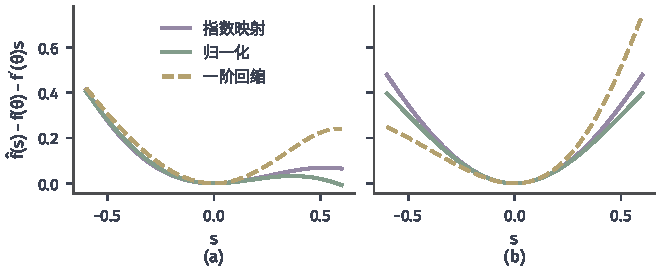
\includegraphics[width=112.0mm]{figures/05-optimization/06-constrained-optimization/matplotlib/mfo-pullback-curvature/figure.pdf}
 \caption{圆周上目标扣除一阶项后的拉回$\hat{f}(s)-\varphi(\theta)-\varphi'(\theta)s$。紫线、绿线、黄虚线分别对应指数映射、归一化与一阶回缩$\theta+s+s^2/2$。(a)~非驻点$\theta=\pi/6$，黄虚线在零点的曲率明显更大。(b)~驻点$\theta=0$，三条曲线在零点处曲率相同。}
 \label{fig:mfo-pullback-curvature}
\end{BookInlineFigure}

\paragraph{用拉回评价候选步}
式~\eqref{eq:mfo-pullback-grad}和式~\eqref{eq:mfo-pullback-hess}支持下面这个切空间二次模型：
\begin{equation}
 m_{\bm{x}}(\bm{v})=f(\bm{x})+\langle\operatorname{grad}f(\bm{x}),\bm{v}\rangle+\frac12\langle\bm{v},\operatorname{Hess}f(\bm{x})[\bm{v}]\rangle.
 \label{eq:mfo-model}
\end{equation}

在贯穿例的方向上核对。沿$s\bm{E}_2$，切向曲率是
\[
 \langle\bm{E}_2,(\bm{A}-q\bm{I})\bm{E}_2\rangle=\frac{22}{9}-\frac{16}{9}=\frac23,
\]
模型是
\[
 m(s\bm{E}_2)=\frac89-\frac89s+\frac13s^2.
\]

用式~\eqref{eq:mfo-pullback-line}减去模型，分子通分后得到
\[
 \hat{f}_{\bm{x}^{(0)}}(s\bm{E}_2)-m(s\bm{E}_2)=\frac{8s^3-3s^4}{9(1+s^2)}.
\]
误差是$s^3$量级，这正是二阶回缩的效果。$s=0.1$时误差约为$8.5\times10^{-4}$，$s=1$时误差是$\tfrac{5}{18}$，模型已不可信，这是信赖域要处理的问题。

\subsection{向量搬运}
\label{sec:mfo-transport}

\paragraph{为什么需要搬运}
共轭梯度要把上一轮的方向和当前梯度相加，拟Newton要算两点梯度之差。欧氏空间里这些都是普通的加减法，流形上却有一个类型错误：旧向量在$T_{\bm{x}}M$中，新向量在$T_{\bm{y}}M$中，两者属于不同的线性空间。

在球面上，不同点的切平面是不同的平面，直接相加得到的向量一般不再切于任何一点。例如$\bm{x}^{(0)}$和$\bm{x}^{(1)}$处的两个切向量之和，通常与$\bm{x}^{(1)}$有非零内积。需要先把旧向量搬到新切空间。

\begin{definition}[向量搬运]
 \label{def:mfo-vector-transport}
 伴随回缩$R$的\term{向量搬运}（vector transport）是一族映射，对$\bm{x}\in M$和$\bm{\eta}\in T_{\bm{x}}M$给出线性映射$\mathcal{T}_{\bm{\eta}}$，它把$T_{\bm{x}}M$映到点$R_{\bm{x}}(\bm{\eta})$的切空间，且随$(\bm{x},\bm{\eta})$光滑变化，并满足$\mathcal{T}_{\bm{0}}=\mathrm{id}$。
\end{definition}

定义只要求三件事：结果落在新切空间中（一致性），对被搬运的向量是线性的，零步时什么也不做。它不要求保持长度和内积。后面需要这些额外性质时，要逐个核对。为了书写简洁，起点$\bm{x}$、终点$\bm{y}=R_{\bm{x}}(\bm{\eta})$明确时，记成$\mathcal{T}_{\bm{x}\to\bm{y}}$。

\paragraph{三种具体搬运}
第一种是\term{投影搬运}（projection transport），把旧向量看作环境空间的向量，投影到新切空间：
\begin{equation}
 \mathcal{T}^{\mathrm{P}}_{\bm{x}\to\bm{y}}(\bm{v})=\bm{P}_{\bm{y}}\bm{v}.
 \label{eq:mfo-projection-transport}
\end{equation}
它只对嵌入子流形可用，计算便宜。正交投影不会增加长度，但一般会减小长度。

第二种是\term{平行移动}（parallel transport），即卷四定义的沿曲线协变导数为零的搬运，它是等距的。球面上沿大圆从$\bm{x}$到$\bm{y}$有闭式：
\begin{equation}
 \mathcal{T}^{\parallel}_{\bm{x}\to\bm{y}}(\bm{v})=\bm{v}-\frac{\langle\bm{x}+\bm{y},\bm{v}\rangle}{1+\langle\bm{x},\bm{y}\rangle}(\bm{x}+\bm{y}).
 \label{eq:mfo-parallel-transport}
\end{equation}
这里要求$\bm{y}\neq-\bm{x}$。

下面验证结果确实切于$\bm{y}$且长度不变。记
\[
 c=\langle\bm{x},\bm{y}\rangle,\qquad a=\langle\bm{x}+\bm{y},\bm{v}\rangle.
\]

由$\bm{v}\perp\bm{x}$有$\langle\bm{y},\bm{v}\rangle=a$，又$\langle\bm{x}+\bm{y},\bm{y}\rangle=1+c$，于是
\[
 \langle\bm{y},\mathcal{T}^{\parallel}\bm{v}\rangle=a-\frac{a}{1+c}(1+c)=0.
\]

再用$\lVert\bm{x}+\bm{y}\rVert_2^2=2+2c$算长度：
\[
 \lVert\mathcal{T}^{\parallel}\bm{v}\rVert_2^2=\lVert\bm{v}\rVert_2^2-\frac{2a^2}{1+c}+\frac{a^2(2+2c)}{(1+c)^2}=\lVert\bm{v}\rVert_2^2.
\]

第三种是\term{微分回缩}（differentiated retraction），直接用回缩曲线的速度：
\[
 \mathcal{T}^{\mathrm{D}}_{\bm{\eta}}(\bm{v})=\frac{\mathrm{d}}{\mathrm{d}t}R_{\bm{x}}(\bm{\eta}+t\bm{v})\Big|_{t=0}.
\]
它的好处是下一节的线搜索导数恰好用这个向量。球面归一化沿搜索方向$\bm{d}$，设$\bm{y}=R_{\bm{x}}(\alpha\bm{d})$，$r=\lVert\bm{x}+\alpha\bm{d}\rVert_2$，求导得到
\[
 \frac{\mathrm{d}}{\mathrm{d}\tau}R_{\bm{x}}\bigl((\alpha+\tau)\bm{d}\bigr)\Big|_{\tau=0}=\frac{1}{r}\bm{P}_{\bm{y}}\bm{d}.
\]
所以此时投影搬运与微分回缩只差一个正的倍数$r$。

\paragraph{搬运结果的比较}
图~\ref{fig:mfo-transport}对比了切向量在两点之间的搬运。把$\bm{v}$平移到$\bm{y}$得到的副本并不切于球面（灰色虚线）。投影把副本垂直压到切平面上，长度变短；平行移动沿大圆旋转切平面，长度不变。

\begin{BookInlineFigure}
 \centering
 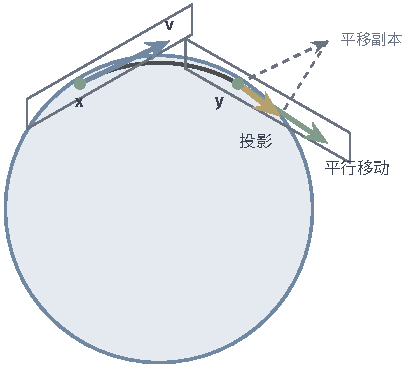
\includegraphics[width=70.0mm]{figures/05-optimization/06-constrained-optimization/tikz/mfo-transport/figure.pdf}
 \caption{把切向量$\bm{v}$（蓝）从$\bm{x}$搬到$\bm{y}$。深灰弧是连接两点的大圆，两个方框是切平面。灰色虚线箭头是平移的副本，不切于球面。黄箭头是投影结果，长度缩短；绿箭头是平行移动结果，长度与$\bm{v}$相同。}
 \label{fig:mfo-transport}
\end{BookInlineFigure}

用贯穿例算一次。第~\ref{sec:mfo-rgd}节将得到$\bm{x}^{(1)}\approx(0.8418,0.5388,-0.0337)^\top$，它与起点的内积约为$0.9091$。把基向量$\bm{E}_1,\bm{E}_2$搬到$\bm{x}^{(1)}$，投影的结果范数约为$0.9949$和$0.9147$，内积约为$0.0408$，平行移动的结果仍是标准正交的。

投影缩短的量取决于向量与连线方向的夹角。沿大圆方向的向量缩短最多，缩短比例等于两点内积。负梯度方向恰好是大圆方向，$\lVert\bm{g}^{(0)}\rVert_2\approx0.9162$的向量投影后长度约为$0.8330$，比值$0.9091$。

因此投影搬运不是等距的：它让向量落进了新切空间，但没有保持内积。若$\bm{y}\perp\bm{x}$，投影还会把沿连线方向的向量压成零，这时映射不可逆。表~\ref{tab:mfo-transport-compare}列出后面的算法需要核对的性质。

\begin{BookInlineTable}
 \centering
 \caption{三种搬运的性质，以球面归一化回缩为例。可逆一栏的$c=\langle\bm{x},\bm{y}\rangle$；一般流形上的平行移动要解常微分方程。}
 \label{tab:mfo-transport-compare}
 \begin{tabular}{llll}
  \toprule
  搬运 & 长度 & 可逆 & 代价\\
  \midrule
  投影 & 一般缩短 & 需$c\neq0$ & $O(n)$\\
  平行移动 & 保持 & 是 & $O(n)$\\
  微分回缩 & 沿步方向缩到$1/r^2$倍 & 需$c\neq0$ & $O(n)$\\
  \bottomrule
 \end{tabular}
\end{BookInlineTable}

\section{一阶方法}
\label{sec:mfo-first-order}

三种几何运算齐备后，先看只用一阶信息的方法。于是要问：负切向梯度加回缩为什么能下降，步长如何选择，以及搬运历史方向怎样加快收敛又带来了哪些新的检查项？

\subsection{黎曼梯度下降}
\label{sec:mfo-rgd}

\paragraph{主要思想}
\term{黎曼梯度下降}（Riemannian gradient descent）在当前切空间中沿负梯度取步，再用回缩回到流形：
\begin{equation}
 \bm{x}^{(t+1)}=R_{\bm{x}^{(t)}}\bigl(-\alpha^{(t)}\bm{g}^{(t)}\bigr),\qquad\bm{g}^{(t)}=\operatorname{grad}f(\bm{x}^{(t)}).
 \label{eq:mfo-rgd}
\end{equation}

为什么这一步能下降？记$\phi(\alpha)=\hat{f}_{\bm{x}}(-\alpha\bm{g})$，这是一个普通的一元函数。由式~\eqref{eq:mfo-pullback-grad}，
\[
 \phi'(0)=\langle\operatorname{grad}f(\bm{x}),-\bm{g}\rangle=-\lVert\bm{g}\rVert_2^2<0.
\]
所以只要$\bm{g}\neq\bm{0}$，足够小的步长一定使目标下降。这个结论只用了回缩的一阶一致性，不需要二阶回缩。

步长的选择与欧氏情形完全平行，只是把比较对象换成拉回函数。Armijo条件要求
\begin{equation}
 f\bigl(R_{\bm{x}}(-\alpha\bm{g})\bigr)\leq f(\bm{x})-c_1\alpha\lVert\bm{g}\rVert_2^2.
 \label{eq:mfo-armijo}
\end{equation}
下降的检验必须针对回缩后的点，切平面上的点$\bm{x}-\alpha\bm{g}$根本不可行，其函数值没有意义。

\needspace{6\baselineskip}
\paragraph{变量}
\begin{itemize}
 \item $\bm{x}^{(t)}\in\mathbb{R}^3$：球面上的当前点，长度为一。
 \item $q^{(t)}$：Rayleigh商的取值，标量。
 \item $\bm{g}^{(t)}$：黎曼梯度，与$\bm{x}^{(t)}$垂直的三维向量。
 \item $\alpha$：当前试探步长；$c_1=\tfrac14$是Armijo常数，缩减因子取$\tfrac12$。
\end{itemize}

\paragraph{初始化}
取$\bm{x}^{(0)}$，初始试探步长$\alpha_0=1$，停止容差$\lVert\bm{g}^{(t)}\rVert_2\leq10^{-6}$。例中$\bm{x}^{(0)}=\tfrac13(2,2,1)^\top$，$f(\bm{x}^{(0)})=\tfrac89$。

\needspace{6\baselineskip}
\paragraph{每轮更新}
\begin{enumerate}
 \item 由式~\eqref{eq:mfo-rayleigh-grad}算$\bm{g}^{(t)}$。例中第$0$轮已算得
 \[
  \bm{g}^{(0)}=\frac{1}{27}(-14,4,20)^\top,\qquad\lVert\bm{g}^{(0)}\rVert_2^2=\frac{68}{81}.
 \]

 \item 令$\alpha=\alpha_0$，按式~\eqref{eq:mfo-sphere-retraction}算试探点，并检验式~\eqref{eq:mfo-armijo}，不满足时$\alpha$减半。例中第$0$轮先试$\alpha=1$：
 \[
  \bm{x}^{(0)}-\bm{g}^{(0)}=\frac{1}{27}(32,14,-11)^\top.
 \]
 归一化后的点是$(0.8738,0.3823,-0.3004)^\top$，目标值$0.7084$，下降$0.1805$，低于要求的$\tfrac14\cdot\tfrac{68}{81}\approx0.2099$，拒绝。

 \item 例中减半后试$\alpha=\tfrac12$，得到
 \[
  \bm{x}^{(0)}-\tfrac12\bm{g}^{(0)}=\frac{1}{27}(25,16,-1)^\top.
 \]
 由勾股定理，长度的平方是$1+\tfrac14\cdot\tfrac{68}{81}=\tfrac{98}{81}$，长度是$\tfrac{7\sqrt2}{9}$。

 \item 接受时令$\bm{x}^{(t+1)}$为该试探点。例中
 \[
  \bm{x}^{(1)}=\frac{(25,16,-1)^\top}{21\sqrt2}\approx(0.8418,0.5388,-0.0337)^\top.
 \]
 目标值$0.6468$，下降$0.2421$，超过要求的$0.1049$，接受。
\end{enumerate}

图~\ref{fig:mfo-rgd-step}画出这一轮的几何：两个候选点都在切平面上，沿径向回到球面后才可以比较。

\begin{BookInlineFigure}
 \centering
 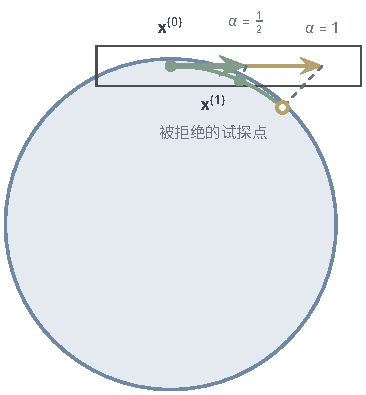
\includegraphics[width=62.0mm]{figures/05-optimization/06-constrained-optimization/tikz/mfo-rgd-step/figure.pdf}
 \caption{第$0$轮迭代的几何，视线接近垂直于$\bm{x}^{(0)}$与$\bm{g}^{(0)}$所在的平面。方框是切平面的一块，黄箭头和绿箭头分别是$\alpha=1$和$\alpha=\tfrac12$的切向步，虚线是归一化回缩。空心点未通过Armijo检验，绿点$\bm{x}^{(1)}$通过。}
 \label{fig:mfo-rgd-step}
\end{BookInlineFigure}

第$1$轮算得
\[
 \bm{g}^{(1)}\approx(-0.2472,0.3805,-0.0911)^\top,\qquad\lVert\bm{g}^{(1)}\rVert_2^2\approx0.2142.
\]
$\alpha=1$的试探点是$(0.9883,0.1436,0.0521)^\top$，目标值$0.5144$，下降$0.1324$，超过要求的$0.0536$，接受。

第$2$轮$\lVert\bm{g}^{(2)}\rVert_2^2\approx0.0443$。$\alpha=1$的试探点目标值$0.5152$，反而上升，拒绝；$\alpha=\tfrac12$的试探点目标值$0.5036$，下降$0.0107$，超过要求的$0.0055$，接受。表~\ref{tab:mfo-rgd-run}汇总前几轮。

\begin{BookInlineTable}
 \centering
 \caption{贯穿例的黎曼梯度下降，回溯线搜索。}
 \label{tab:mfo-rgd-run}
 \begin{tabular}{lllll}
  \toprule
  $t$ & $\bm{x}^{(t)}$ & $f(\bm{x}^{(t)})$ & $\lVert\bm{g}^{(t)}\rVert_2$ & 接受的$\alpha$\\
  \midrule
  $0$ & $(0.6667,0.6667,0.3333)$ & $0.8889$ & $0.9162$ & $0.5$\\
  $1$ & $(0.8418,0.5388,-0.0337)$ & $0.6468$ & $0.4628$ & $1$\\
  $2$ & $(0.9883,0.1436,0.0521)$ & $0.5144$ & $0.2104$ & $0.5$\\
  $3$ & $(0.9970,0.0735,-0.0252)$ & $0.5036$ & $0.1051$ & $0.5$\\
  $4$ & $(0.9992,0.0369,0.0125)$ & $0.5009$ & $0.0526$ & $0.5$\\
  \bottomrule
 \end{tabular}
\end{BookInlineTable}

末尾几轮梯度范数每轮减半。这有明确的来由：$\bm{e}_1$处切向曲率是$1$和$3$，局部迭代相当于$\bm{v}\mapsto(\bm{I}-\alpha\bm{H})\bm{v}$，$\alpha=\tfrac12$时两个因子是$\tfrac12$和$-\tfrac12$。这也解释了第三个坐标的符号交替。当$\lVert\bm{g}^{(t)}\rVert_2\leq10^{-6}$时停止，最终得到$\bm{x}^{(T)}\approx\bm{e}_1$。

图~\ref{fig:mfo-rgd-path}是球面上的路径，图~\ref{fig:mfo-rgd-convergence}是收敛曲线。固定步长$\alpha=\tfrac29$的路径更平缓，但每轮的收缩因子是$1-\tfrac29=\tfrac79$，慢得多。

\begin{BookInlineFigure}
 \centering
 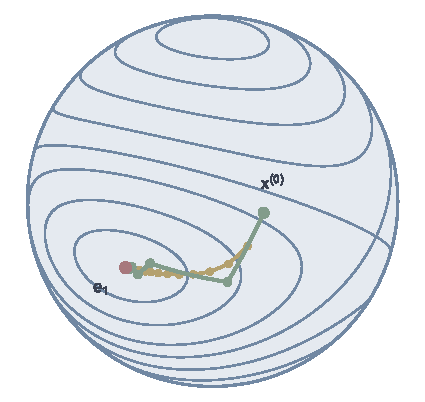
\includegraphics[width=72.0mm]{figures/05-optimization/06-constrained-optimization/matplotlib/mfo-rgd-path/figure.pdf}
 \caption{球面上的迭代路径，蓝线是目标的等高线。绿色为回溯线搜索（$c_1=\tfrac14$），黄色为固定步长$\alpha=\tfrac29$，点之间用大圆弧连接，红点是极小点。}
 \label{fig:mfo-rgd-path}
\end{BookInlineFigure}

\begin{BookInlineFigure}
 \centering
 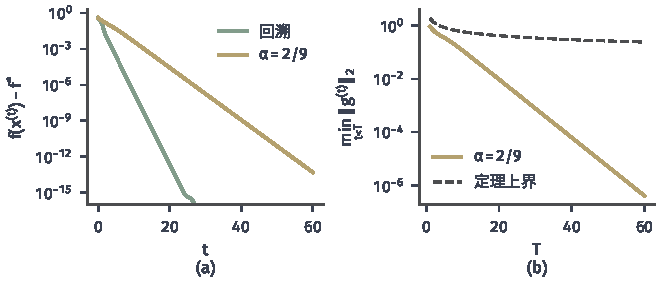
\includegraphics[width=112.0mm]{figures/05-optimization/06-constrained-optimization/matplotlib/mfo-rgd-convergence/figure.pdf}
 \caption{贯穿例上的收敛。(a)~目标误差，绿色回溯，黄色固定步长$\tfrac29$。(b)~固定步长下至第$T$轮为止的最小梯度范数（黄）与定理~\ref{thm:mfo-rgd-rate}给出的上界（灰虚线，$L=\tfrac92$）。上界有效，但对这个问题偏松。}
 \label{fig:mfo-rgd-convergence}
\end{BookInlineFigure}

\paragraph{收敛性}
欧氏分析的关键是下降引理，流形上只需要把它改写成对拉回函数的假设。这个假设是下面的上界，称为拉回的$L$光滑性：对所考虑的$\bm{x}$和$\bm{v}$，
\begin{equation}
 f(R_{\bm{x}}(\bm{v}))\leq f(\bm{x})+\langle\operatorname{grad}f(\bm{x}),\bm{v}\rangle+\frac L2\lVert\bm{v}\rVert_2^2.
 \label{eq:mfo-pullback-smooth}
\end{equation}

\begin{theorem}[黎曼梯度下降的残差界]
 \label{thm:mfo-rgd-rate}
 设$f$在$M$上有下界$f^\star$，并且式~\eqref{eq:mfo-pullback-smooth}对所有$\bm{x}\in M$和$\bm{v}\in T_{\bm{x}}M$成立。取固定步长$\alpha=1/L$，则
 \begin{equation}
  \min_{0\leq t<T}\lVert\bm{g}^{(t)}\rVert_2\leq\sqrt{\frac{2L\bigl(f(\bm{x}^{(0)})-f^\star\bigr)}{T}}.
  \label{eq:mfo-rgd-rate}
 \end{equation}
 改用初始步长$\alpha_0$、缩减因子$\beta\in(0,1)$的Armijo回溯时，接受的步长不小于
 \begin{equation}
  \underline{\alpha}=\min\Bigl\{\alpha_0,\ \frac{2\beta(1-c_1)}{L}\Bigr\},
  \label{eq:mfo-armijo-floor}
 \end{equation}
 每轮下降至少$c_1\underline{\alpha}\lVert\bm{g}^{(t)}\rVert_2^2$。
\end{theorem}

\begin{proof}
 取$\bm{v}=-\alpha\bm{g}^{(t)}$代入式~\eqref{eq:mfo-pullback-smooth}，$\alpha=1/L$时得到
 \[
  f(\bm{x}^{(t+1)})\leq f(\bm{x}^{(t)})-\frac{1}{L}\lVert\bm{g}^{(t)}\rVert_2^2+\frac{1}{2L}\lVert\bm{g}^{(t)}\rVert_2^2=f(\bm{x}^{(t)})-\frac{1}{2L}\lVert\bm{g}^{(t)}\rVert_2^2.
 \]

 对$t=0,\ldots,T-1$求和，左边相消，再用$f(\bm{x}^{(T)})\geq f^\star$，于是
 \[
  \frac{1}{2L}\sum_{t=0}^{T-1}\lVert\bm{g}^{(t)}\rVert_2^2\leq f(\bm{x}^{(0)})-f^\star.
 \]
 和式不小于$T$乘最小项，整理得式~\eqref{eq:mfo-rgd-rate}。

 再看回溯。由式~\eqref{eq:mfo-pullback-smooth}，只要$\alpha\leq2(1-c_1)/L$，就有
 \[
  f(R_{\bm{x}}(-\alpha\bm{g}))\leq f(\bm{x})-\alpha\Bigl(1-\frac{L\alpha}{2}\Bigr)\lVert\bm{g}\rVert_2^2\leq f(\bm{x})-c_1\alpha\lVert\bm{g}\rVert_2^2,
 \]
 Armijo条件成立。若初始步长被拒绝，则最后一次被拒绝的步长大于$2(1-c_1)/L$，接受的步长至少是它的$\beta$倍，所以接受的步长不小于$\underline{\alpha}$。
\end{proof}

定理的结论是梯度范数变小，这里的量不是到极小点的距离，也没有说收敛到全局极小。常数$L$依赖回缩：同一目标换一个回缩，上界~\eqref{eq:mfo-pullback-smooth}中的常数也要重新估计。

对紧流形、光滑目标和光滑回缩，式~\eqref{eq:mfo-pullback-smooth}在切向量长度有上界的范围内自动成立，因为拉回的二阶导数在紧集上有界。贯穿例的归一化回缩可以把常数算出来，而且不限长度。

\begin{lemma}[球面Rayleigh商的光滑常数]
 \label{lem:mfo-sphere-l}
 设$\bm{A}$对称，最小、最大特征值为$\lambda_1,\lambda_n$，$f(\bm{x})=\tfrac12\bm{x}^\top\bm{A}\bm{x}$，回缩为式~\eqref{eq:mfo-sphere-retraction}。则式~\eqref{eq:mfo-pullback-smooth}对所有$\bm{x}\in S^{n-1}$，$\bm{v}\perp\bm{x}$成立，常数可取
 \begin{equation}
  L=\frac32(\lambda_n-\lambda_1).
  \label{eq:mfo-sphere-l}
 \end{equation}
\end{lemma}

\begin{proof}
 记$s=\lVert\bm{v}\rVert_2^2$。因为$\bm{v}\perp\bm{x}$，切向梯度与$\bm{v}$的内积等于$\bm{x}^\top\bm{A}\bm{v}$。把回缩代入后通分，得到
 \[
  f(R_{\bm{x}}(\bm{v}))-f(\bm{x})-\langle\bm{g},\bm{v}\rangle=\frac{\tfrac12\bm{v}^\top\bm{A}\bm{v}-\tfrac12qs-s\,\bm{x}^\top\bm{A}\bm{v}}{1+s}.
 \]

 分子前两项满足
 \[
  \frac12\bm{v}^\top\bm{A}\bm{v}-\frac12qs\leq\frac12(\lambda_n-\lambda_1)s,
 \]
 这里用了$\bm{v}^\top\bm{A}\bm{v}\leq\lambda_ns$，$q\geq\lambda_1$。分母不小于一，这一部分的贡献不超过$\tfrac12(\lambda_n-\lambda_1)s$。

 第三项用Cauchy--Schwarz不等式和$\sqrt{s}/(1+s)\leq\tfrac12$，得到
 \[
  \frac{s\,\lvert\langle\bm{g},\bm{v}\rangle\rvert}{1+s}\leq s\lVert\bm{g}\rVert_2\frac{\sqrt{s}}{1+s}\leq\frac12\lVert\bm{g}\rVert_2\,s.
 \]

 最后界住梯度。因为$(\bm{A}-\lambda_1\bm{I})(\lambda_n\bm{I}-\bm{A})$半正定，在$\bm{x}$上取二次型并整理，得到
 \[
  \lVert\bm{g}\rVert_2^2=\bm{x}^\top\bm{A}^2\bm{x}-q^2\leq(q-\lambda_1)(\lambda_n-q)\leq\Bigl(\frac{\lambda_n-\lambda_1}{2}\Bigr)^2.
 \]
 把三部分合并，上界是
 \[
  \frac12(\lambda_n-\lambda_1)s+\frac14(\lambda_n-\lambda_1)s=\frac12Ls,\qquad L=\frac32(\lambda_n-\lambda_1),
 \]
 这正是式~\eqref{eq:mfo-pullback-smooth}所需的形式。
\end{proof}

贯穿例中$\lambda_n-\lambda_1=3$，所以$L=\tfrac92$，$1/L=\tfrac29$，这是图中固定步长的来历。随机采样$20$万组$(\bm{x},\bm{v})$，式~\eqref{eq:mfo-pullback-smooth}所需常数的最大值约为$2.98$，说明这个界偏保守，但安全。

\paragraph{每轮成本}
梯度、投影和回缩的每轮代价应当一起计算。球面上一次$\bm{A}$乘向量算出$\bm{g}^{(t)}$，投影和归一化都是$O(n)$，线搜索的每次试探还要一次目标计算。若$\bm{A}$是大规模稀疏矩阵，主要开销就是$\bm{A}$乘向量。$\mathrm{St}(k,n)$上每轮要做$\bm{A}\bm{X}$、投影和$O(nk^2)$的QR分解，$k$较大时回缩的比重不能忽略。

\subsection{黎曼共轭梯度}
\label{sec:mfo-rcg}

\paragraph{主要思想}
第~\ref{chap:first-order-methods}章的非线性共轭梯度把上一轮方向与当前负梯度相加，得到比负梯度更好的方向。流形上上一轮方向$\bm{d}^{(t)}$在$T_{\bm{x}^{(t)}}M$中，需要先搬到新切空间。\term{黎曼共轭梯度}（Riemannian conjugate gradient）的方向更新是
\begin{equation}
 \bm{d}^{(t+1)}=-\bm{g}^{(t+1)}+\beta^{(t+1)}\mathcal{T}_{\bm{x}^{(t)}\to\bm{x}^{(t+1)}}\bigl(\bm{d}^{(t)}\bigr).
 \label{eq:mfo-rcg-direction}
\end{equation}

系数$\beta$也要用同一切空间中的量。Fletcher--Reeves形式只用两个梯度的范数，范数是各自切空间内算的，不需要搬运：
\begin{equation}
 \beta_{\mathrm{FR}}^{(t+1)}=\frac{\lVert\bm{g}^{(t+1)}\rVert_2^2}{\lVert\bm{g}^{(t)}\rVert_2^2}.
 \label{eq:mfo-beta-fr}
\end{equation}

Polak--Ribière形式要算梯度之差，旧梯度必须先搬过去：
\begin{equation}
 \beta_{\mathrm{PR}}^{(t+1)}=\frac{\bigl\langle\bm{g}^{(t+1)},\ \bm{g}^{(t+1)}-\mathcal{T}_{\bm{x}^{(t)}\to\bm{x}^{(t+1)}}(\bm{g}^{(t)})\bigr\rangle}{\lVert\bm{g}^{(t)}\rVert_2^2}.
 \label{eq:mfo-beta-pr}
\end{equation}
实际常取$\max\{0,\beta_{\mathrm{PR}}\}$，这称为PR+，系数为零时自动回到负梯度方向。

\needspace{6\baselineskip}
\paragraph{变量}
\begin{itemize}
 \item $\bm{x}^{(t)}$、$\bm{g}^{(t)}$：当前点与黎曼梯度，均为三维向量。
 \item $\bm{d}^{(t)}$：搜索方向，切于$\bm{x}^{(t)}$。
 \item $\widetilde{\bm{d}}$：上一轮方向搬运到新切空间后的向量。
 \item $\beta$：组合系数；线搜索常数$c_1=\tfrac14$，试探步长从$1$开始减半。
\end{itemize}

\paragraph{初始化}
令$\bm{d}^{(0)}=-\bm{g}^{(0)}$，搬运取投影~\eqref{eq:mfo-projection-transport}。例中第$0$轮与梯度下降相同，接受$\alpha=\tfrac12$，得到$\bm{x}^{(1)}$。

\needspace{6\baselineskip}
\paragraph{每轮更新}
\begin{enumerate}
 \item 用式~\eqref{eq:mfo-armijo}的形式沿$\bm{d}^{(t)}$回溯，把右端的$-\lVert\bm{g}\rVert_2^2$换成$\langle\bm{g}^{(t)},\bm{d}^{(t)}\rangle$，得到$\bm{x}^{(t+1)}$。

 \item 计算新梯度。例中第$1$轮
 \[
  \bm{g}^{(1)}\approx(-0.2472,0.3805,-0.0911)^\top.
 \]

 \item 由式~\eqref{eq:mfo-projection-transport}搬运旧方向。例中$\bm{d}^{(0)}=-\bm{g}^{(0)}$，
 \[
  \widetilde{\bm{d}}=\bm{P}_{\bm{x}^{(1)}}\bm{d}^{(0)}\approx(0.1973,-0.3537,-0.7279)^\top.
 \]

 \item 由式~\eqref{eq:mfo-beta-fr}算系数。例中
 \[
  \beta_{\mathrm{FR}}^{(1)}=\frac{0.2142}{0.8395}\approx0.2552.
 \]

 \item 由式~\eqref{eq:mfo-rcg-direction}组合新方向。例中
 \[
  \bm{d}^{(1)}\approx(0.2975,-0.4708,-0.0946)^\top.
 \]

 \item 检查下降性：若$\langle\bm{g}^{(t+1)},\bm{d}^{(t+1)}\rangle\geq0$，重启，令$\bm{d}^{(t+1)}=-\bm{g}^{(t+1)}$。例中内积约为$-0.2441<0$，不需要重启。
\end{enumerate}

例中第$1$轮沿$\bm{d}^{(1)}$试$\alpha=1$，得到$\bm{x}^{(2)}\approx(0.9920,0.0592,-0.1117)^\top$，目标值$0.5205$，下降$0.1264$，超过要求的$0.0610$，接受。

第$2$轮算得$\beta^{(2)}_{\mathrm{FR}}\approx0.5326$，方向$\bm{d}^{(2)}\approx(0.0523,-0.3163,0.2967)^\top$。$\alpha=1$和$\alpha=\tfrac12$都未通过，$\alpha=\tfrac14$通过，得到目标值$0.5023$。当$\lVert\bm{g}^{(t)}\rVert_2\leq10^{-6}$时结束，最终得到$\bm{x}^{(T)}\approx\pm\bm{e}_1$。

三维问题上共轭梯度几乎没有优势：例中第$2$轮的目标值$0.5205$还略高于梯度下降的$0.5144$。历史方向的收益要在维数更高、条件数更大的问题上才显现。图~\ref{fig:mfo-rcg-compare}取$n=200$的问题，迭代到$\lVert\bm{g}\rVert_2\leq10^{-6}$为止，使用精确的拉回线搜索，PR+用了约$158$轮，FR用了约$284$轮。

\begin{BookInlineFigure}
 \centering
 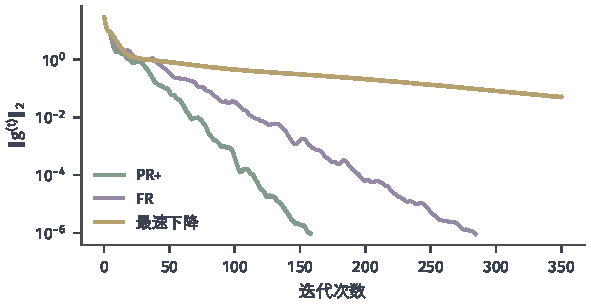
\includegraphics[width=100.0mm]{figures/05-optimization/06-constrained-optimization/matplotlib/mfo-rcg-compare/figure.pdf}
 \caption{$n=200$，$\bm{A}$的特征值在$1$到$100$之间等距，随机起点固定，球面上沿拉回函数作精确线搜索，用投影搬运。绿、紫分别为PR+与FR，黄色为最速下降。纵轴是黎曼梯度范数，最速下降在$350$轮内远未达到容差。}
 \label{fig:mfo-rcg-compare}
\end{BookInlineFigure}

\paragraph{需要核对的条件}
欧氏共轭梯度的保证不能直接照搬，有四项需要逐一核对。第一是方向的下降性。对式~\eqref{eq:mfo-rcg-direction}与$\bm{g}^{(t+1)}$作内积，得到
\[
 \langle\bm{g}^{(t+1)},\bm{d}^{(t+1)}\rangle=-\lVert\bm{g}^{(t+1)}\rVert_2^2+\beta^{(t+1)}\langle\bm{g}^{(t+1)},\mathcal{T}(\bm{d}^{(t)})\rangle.
\]
右端第二项若为正且较大，方向就不是下降方向。

第二是线搜索与搬运是否配套。欧氏情形下强Wolfe条件控制的正是$\langle\bm{g}^{(t+1)},\bm{d}^{(t)}\rangle$的大小。流形上线搜索控制的是一元函数的导数
\[
 \phi'(\alpha)=\bigl\langle\bm{g}^{(t+1)},\mathcal{T}^{\mathrm{D}}_{\alpha\bm{d}}(\bm{d})\bigr\rangle,
\]
它使用的是微分回缩。若方向更新用了另一种搬运，线搜索就控制不到上式第二项。

球面归一化时这个问题比较简单：第~\ref{sec:mfo-transport}节已指出投影搬运只差一个正因子$r$。例中$\langle\bm{g}^{(1)},\widetilde{\bm{d}}\rangle\approx-0.1171$，而$r=\tfrac{7\sqrt2}{9}$，所以$\phi'(\tfrac12)\approx-0.1064$。这个配套关系是例子的特殊之处，一般不成立。

第三是搬运的范数。关于FR的全局收敛分析通常要求搬运后的方向不比原方向长，否则可以用一个缩放因子修正。投影搬运满足这一点，平行移动也满足。证明需要把Zoutendijk型的求和论证搬到流形上，篇幅较长，读者可查阅关于黎曼共轭梯度收敛的专门文献。其结论大意是：强Wolfe条件和不增长的搬运使FR方向保持下降，并且$\liminf_{t\to\infty}\lVert\bm{g}^{(t)}\rVert_2=0$。

第四是重启。一方面下降性检查失败时需要重启；另一方面在非二次目标上旧方向会过时，常用的做法是每隔$\dim M$轮或连续两轮梯度明显不正交时重启。FR、PR+、搬运、线搜索的组合不同，保证也不同，任意组合不能默认继承欧氏结论。

\section{二阶方法}
\label{sec:mfo-second-order}

一阶方法在贯穿例上每轮把误差减半，曲率矩阵的条件数变大时会更慢。切空间里的曲率信息能否换来一个更准确的步？接下来要弄清：这个线性子问题怎样写出，什么时候它的解值得采用？

需要分清三个判断，它们常常被混为一谈。模型非退化说的是线性子问题有唯一解，方向下降说的是这个解确实使目标减小，局部极小说的是所趋向的点是极小点。表~\ref{tab:mfo-three-judgments}用第~\ref{chap:second-order-methods}章的语言把它们并列。

\begin{BookInlineTable}
 \centering
 \caption{曲率算子的三种判断，$\bm{H}$是当前点的黎曼Hessian。}
 \label{tab:mfo-three-judgments}
 \begin{tabular}{lll}
  \toprule
  判断 & 条件 & 不保证什么\\
  \midrule
  模型非退化 & $\bm{H}$可逆 & 解是下降方向\\
  方向下降 & $\bm{H}$在切空间上正定即可 & 趋向极小点的全局性\\
  局部极小 & 驻点处$\bm{H}$正定 & 全局极小\\
  \bottomrule
 \end{tabular}
\end{BookInlineTable}

\subsection{黎曼Newton法}
\label{sec:mfo-newton}

\paragraph{主要思想}
由第~\ref{sec:mfo-pullback}节，模型~\eqref{eq:mfo-model}是拉回函数在零点的二阶近似。令模型的梯度为零，就得到切空间内的线性方程，\term{黎曼Newton法}（Riemannian Newton method）解这个方程再回缩：
\begin{equation}
 \operatorname{Hess}f(\bm{x}^{(t)})[\bm{v}^{(t)}]=-\bm{g}^{(t)},\quad\bm{v}^{(t)}\in T_{\bm{x}^{(t)}}M,
 \qquad
 \bm{x}^{(t+1)}=R_{\bm{x}^{(t)}}(\bm{v}^{(t)}).
 \label{eq:mfo-newton}
\end{equation}
未知量被限制在切空间中，这正是与欧氏Newton法不同的地方。方程的维数是$\dim M$，而不是环境空间的维数。

球面Rayleigh商上这个方程可以显式解出。由式~\eqref{eq:mfo-rayleigh-grad}和式~\eqref{eq:mfo-rayleigh-hess}，方程写成
\[
 \bm{P}_{\bm{x}}\bigl(\bm{A}\bm{v}\bigr)-q\bm{v}=-\bigl(\bm{A}\bm{x}-q\bm{x}\bigr),\qquad\bm{v}\perp\bm{x}.
\]

去掉投影时要补上一个沿$\bm{x}$的未知倍数$\lambda$。设$\bm{A}-q\bm{I}$可逆，移项后得到
\[
 (\bm{A}-q\bm{I})(\bm{x}+\bm{v})=\lambda\bm{x},\qquad
 \bm{x}+\bm{v}=\lambda(\bm{A}-q\bm{I})^{-1}\bm{x}.
\]

再用$\bm{x}^\top\bm{v}=0$确定$\lambda$，也就是$\bm{x}^\top(\bm{x}+\bm{v})=1$。于是
\begin{equation}
 \bm{x}+\bm{v}=\frac{(\bm{A}-q\bm{I})^{-1}\bm{x}}{\bm{x}^\top(\bm{A}-q\bm{I})^{-1}\bm{x}}.
 \label{eq:mfo-newton-closed}
\end{equation}

归一化之后分母的倍数消失，Newton迭代成为
\begin{equation}
 \bm{x}^{(t+1)}=\pm\frac{(\bm{A}-q^{(t)}\bm{I})^{-1}\bm{x}^{(t)}}{\bigl\lVert(\bm{A}-q^{(t)}\bm{I})^{-1}\bm{x}^{(t)}\bigr\rVert_2},
 \label{eq:mfo-rqi}
\end{equation}
符号由式~\eqref{eq:mfo-newton-closed}决定。这就是经典的Rayleigh商迭代。一个特征值算法，原来是球面上的Newton法加归一化回缩。

\needspace{6\baselineskip}
\paragraph{变量}
\begin{itemize}
 \item $\bm{x}^{(t)}$：球面上的当前点；$q^{(t)}$：Rayleigh商的取值。
 \item $\bm{z}=(\bm{A}-q^{(t)}\bm{I})^{-1}\bm{x}^{(t)}$：三维向量。
 \item $\lambda=1/(\bm{x}^{(t)\top}\bm{z})$：标量，由切向条件确定。
 \item $\bm{v}^{(t)}=\lambda\bm{z}-\bm{x}^{(t)}$：Newton步，切于$\bm{x}^{(t)}$。
\end{itemize}

\paragraph{初始化}
这里换一个更靠近解的起点，理由在后面解释。例中取
\[
 \bm{x}^{(0)}=\frac19(8,4,1)^\top,\qquad q^{(0)}=\frac{64+32+4}{81}=\frac{100}{81}.
\]
停止条件取$\lVert\bm{g}^{(t)}\rVert_2\leq10^{-6}$。

\needspace{6\baselineskip}
\paragraph{每轮更新}
\begin{enumerate}
 \item 计算$\bm{z}$。例中第$0$轮
 \[
  \bm{A}-q^{(0)}\bm{I}=\frac{1}{81}\operatorname{diag}(-19,62,224),
 \]
 所以
 \[
  \bm{z}=\Bigl(-\frac{72}{19},\ \frac{18}{31},\ \frac{9}{224}\Bigr)^\top\approx(-3.7895,\ 0.5806,\ 0.0402)^\top.
 \]

 \item 计算$\lambda$。例中$\bm{x}^{(0)\top}\bm{z}\approx-3.1058$，所以$\lambda\approx-0.3220$。

 \item 由式~\eqref{eq:mfo-newton-closed}得到$\bm{x}+\bm{v}$，由$\bm{v}=\lambda\bm{z}-\bm{x}$读出Newton步。例中
 \[
  \begin{gathered}
  \bm{x}^{(0)}+\bm{v}^{(0)}\approx(1.2201,-0.1870,-0.0129)^\top,\\
  \bm{v}^{(0)}\approx(0.3312,-0.6314,-0.1241)^\top.
  \end{gathered}
 \]

 \item 回缩。例中$\bm{x}^{(1)}\approx(0.9884,-0.1515,-0.0105)^\top$，$\lVert\bm{g}^{(1)}\rVert_2\approx0.1529$。
\end{enumerate}

继续迭代得到表~\ref{tab:mfo-newton-run}。第$3$轮满足停止条件，最终得到$\bm{x}^{(3)}\approx\bm{e}_1$，只用了三次线性方程的求解。

\begin{BookInlineTable}
 \centering
 \caption{从$(8,4,1)^\top/9$出发的黎曼Newton法。最后一列是切空间上$\bm{H}^{(t)}$的特征值。}
 \label{tab:mfo-newton-run}
 \begin{tabular}{lllll}
  \toprule
  $t$ & $\bm{x}^{(t)}$ & $q^{(t)}$ & $\lVert\bm{g}^{(t)}\rVert_2$ & $\bm{H}^{(t)}$的特征值\\
  \midrule
  $0$ & $(0.8889,0.4444,0.1111)$ & $1.2346$ & $0.5036$ & $0.5645,\ 2.7318$\\
  $1$ & $(0.9884,-0.1515,-0.0105)$ & $1.0233$ & $0.1529$ & $0.9538,\ 2.9764$\\
  $2$ & $(1.0000,0.0037,0.0001)$ & $1.0000$ & $3.66\times10^{-3}$ & $1.0000,\ 3.0000$\\
  $3$ & $(1.0000,0.0000,0.0000)$ & $1.0000$ & $4.87\times10^{-8}$ & $1.0000,\ 3.0000$\\
  \bottomrule
 \end{tabular}
\end{BookInlineTable}

\paragraph{局部收敛}
表中的梯度范数几乎是按立方在减小：$0.1529^3\approx3.6\times10^{-3}$，$(3.66\times10^{-3})^3\approx4.9\times10^{-8}$。一般情形的局部结论是平方收敛，这里的立方来自Rayleigh商的特殊结构。

一般结论是：设$\bm{x}^\star$是驻点，$\operatorname{Hess}f(\bm{x}^\star)$可逆，$f$足够光滑，$R$是光滑回缩，则存在$\bm{x}^\star$的邻域，从其中出发的迭代~\eqref{eq:mfo-newton}收敛到$\bm{x}^\star$，至少是平方速度。

严格证明要把迭代写进一张局部坐标图，再逐项控制回缩与坐标化带来的误差，篇幅较长，读者可查阅专门讨论流形优化的著作\scite{math-boumal2023optimization}。机制是这样的：第~\ref{sec:mfo-pullback}节表明，拉回Hessian与黎曼Hessian之差正比于$\lVert\operatorname{grad}f\rVert_2$，在解附近这个差与误差同阶，而一阶量的误差对Newton法只产生平方量级的后果。所以这里任何光滑回缩都行，不必是二阶回缩。

立方的来历可以直接算出。设$\bm{x}=\cos e\,\bm{e}_1+\sin e\,\bm{u}$，$\bm{u}$是$\bm{A}$的另一单位特征向量，特征值$\lambda_u$。Rayleigh商的误差是二阶的：
\[
 q-\lambda_1=(\lambda_u-\lambda_1)\sin^2e.
\]

$(\bm{A}-q\bm{I})^{-1}$把$\bm{e}_1$分量放大$1/(\lambda_1-q)$倍，把$\bm{u}$分量放大$1/(\lambda_u-q)$倍。两个分量的比值给出新的夹角：
\[
 \tan e^{+}=\tan e\cdot\frac{\lvert\lambda_1-q\rvert}{\lvert\lambda_u-q\rvert}=\tan e\cdot\frac{\sin^2e}{\cos^2e}=\tan^3e.
\]
这里用了$\lambda_u-q=(\lambda_u-\lambda_1)\cos^2e$。当$\bm{x}$的误差主要在一个特征方向上时立方律是精确的，这解释了表中系数接近一。

图~\ref{fig:mfo-newton-rate}把这个速度与上一节的梯度下降放在同一张图上。

\begin{BookInlineFigure}
 \centering
 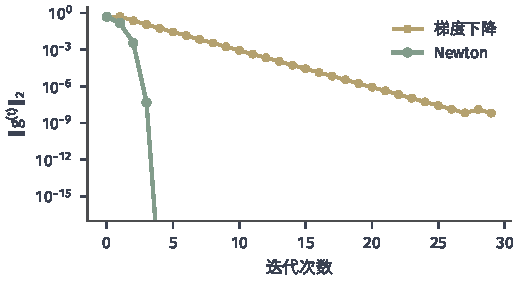
\includegraphics[width=88.0mm]{figures/05-optimization/06-constrained-optimization/matplotlib/mfo-newton-rate/figure.pdf}
 \caption{从同一起点$(8,4,1)^\top/9$出发的黎曼梯度范数。绿线是黎曼Newton法，黄线是回溯线搜索的梯度下降。}
 \label{fig:mfo-newton-rate}
\end{BookInlineFigure}

\paragraph{远离解时}
回到原来的起点$\bm{x}^{(0)}=\tfrac13(2,2,1)^\top$，就能看到为什么上面要换起点。在基$\bm{E}_1,\bm{E}_2$下，$\bm{g}$和$\bm{H}$的坐标表示可由$\bm{A}-q\bm{I}$（对角元为$-\tfrac79,\tfrac29,\tfrac{20}{9}$）算出：
\[
 \bm{g}=\begin{bmatrix}2/9\\-8/9\end{bmatrix},\qquad
 \bm{H}=\begin{bmatrix}1&-10/9\\-10/9&2/3\end{bmatrix},\qquad
 \det\bm{H}=-\frac{46}{81}.
\]
行列式为负，$\bm{H}$的特征值约为$-0.290$和$1.957$，这里模型非退化，但不正定。

解线性方程，得到Newton步的坐标
\[
 \bm{v}=-\bm{H}^{-1}\bm{g}=-\Bigl(\frac{34}{23},\ \frac{26}{23}\Bigr)^\top.
\]

检查方向导数，它是正的：
\[
 \langle\bm{g},\bm{v}\rangle=-\frac29\cdot\frac{34}{23}+\frac89\cdot\frac{26}{23}=\frac{140}{207}>0.
\]
Newton步是上升方向。回缩后的点约为$(-0.274,0.960,0.048)^\top$，目标值从$0.889$升到$0.965$，这个点靠近鞍点$\bm{e}_2$。

这个现象并非偶然。Newton法寻找的是驻点，它对极小点、鞍点和极大点一视同仁。图~\ref{fig:mfo-newton-basin}标出未加保护的Rayleigh商迭代从球面上各点出发时的去向，起点$\bm{x}^{(0)}$恰好落在通往$\bm{e}_2$的区域。

\begin{BookInlineFigure}
 \centering
 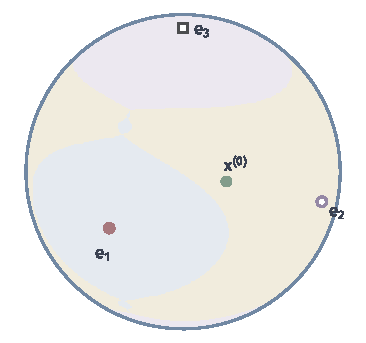
\includegraphics[width=62.0mm]{figures/05-optimization/06-constrained-optimization/matplotlib/mfo-newton-basin/figure.pdf}
 \caption{未加保护的黎曼Newton迭代的去向。每个点的底色表示从该点出发$40$步后趋向哪一对特征向量：浅蓝趋向$\pm\bm{e}_1$，浅黄趋向$\pm\bm{e}_2$，浅紫趋向$\pm\bm{e}_3$。绿点是起点$\bm{x}^{(0)}$，它落在浅黄区域。}
 \label{fig:mfo-newton-basin}
\end{BookInlineFigure}

\subsection{阻尼与非精确求解}
\label{sec:mfo-damped-inexact}

Newton步需要两层保护：方向要下降，步长要合适。规模大的时候还有第三个问题，线性方程不能精确求解。这三件事的思想都来自第~\ref{chap:second-order-methods}章，本节只说明在切空间上有什么变化。

\paragraph{修正曲率}
若$\bm{H}$在切空间上正定，Newton步是下降方向，因为
\[
 \langle\bm{g},\bm{v}\rangle=-\langle\bm{v},\bm{H}[\bm{v}]\rangle<0.
\]
否则就把$\bm{H}$换成$\bm{H}+\tau\bm{I}$，$\tau>0$大到足以使它在切空间上正定。这里的$\bm{I}$是切空间上的恒等算子。

在贯穿例的起点取$\tau=1$，修正后的特征值约为$0.710$和$2.957$，正定。解线性方程得到
\[
 \bm{v}=-(\bm{H}+\bm{I})^{-1}\bm{g}=\Bigl(\frac{5}{17},\ \frac{62}{85}\Bigr)^\top\approx(0.2941,\ 0.7294)^\top.
\]

方向导数约为$-0.583$，确实下降。用$c_1=\tfrac14$做回缩线搜索，试探$\alpha=1$，得到
\[
 R_{\bm{x}^{(0)}}(\bm{v})\approx(0.9833,0.1788,0.0339)^\top,\qquad f\approx0.5177.
\]
下降约$0.371$，超过要求的$0.146$，接受。这一步的目标值比梯度下降第$1$轮的$0.6468$小得多。

Armijo线搜索在这里同样要针对回缩后的点。切向方向下降只保证步足够短时有效，与第~\ref{sec:mfo-rgd}节的道理相同。

\paragraph{用Hessian--向量乘积代替形成矩阵}
当$\dim M$很大时，不可能写出$\bm{H}$的矩阵。Rayleigh商的式~\eqref{eq:mfo-rayleigh-hess}告诉我们，算$\bm{H}[\bm{v}]$只需要一次$\bm{A}$乘向量和一次投影，所以可以用线性共轭梯度法迭代求解式~\eqref{eq:mfo-newton}。

这里的“共轭梯度”要与第~\ref{sec:mfo-rcg}节区分开，表~\ref{tab:mfo-cg-compare}列出区别。内层CG全程在同一个切空间中，解一个线性方程，不需要回缩和搬运。

\begin{BookInlineTable}
 \centering
 \caption{两种共轭梯度。}
 \label{tab:mfo-cg-compare}
 \begin{tabular}{lll}
  \toprule
  & 内层线性CG & 黎曼共轭梯度\\
  \midrule
  解决的问题 & 切空间内的线性方程 & 流形上的非线性优化\\
  所在空间 & 固定的$T_{\bm{x}}M$ & 每轮更换切空间\\
  回缩与搬运 & 不需要 & 每轮都需要\\
  曲率使用 & Hessian--向量乘积 & 不使用\\
  \bottomrule
 \end{tabular}
\end{BookInlineTable}

\paragraph{按切空间的残差设定精度}
线性方程不必解得太准。切空间内的残差是$\bm{r}=\bm{H}[\bm{v}]+\bm{g}$，内层在下述条件满足时停止：
\begin{equation}
 \lVert\bm{r}\rVert_2\leq\eta^{(t)}\lVert\bm{g}^{(t)}\rVert_2.
 \label{eq:mfo-forcing}
\end{equation}
第~\ref{chap:second-order-methods}章的结论在这里同样适用：固定的$\eta<1$一般只给出线性收敛，$\eta^{(t)}\to0$给出超线性收敛，$\eta^{(t)}=O(\lVert\bm{g}^{(t)}\rVert_2)$在解附近恢复平方收敛。

图~\ref{fig:mfo-inexact-newton}是$n=500$的实验。三种规则的总Hessian--向量乘积数分别约为$815$、$815$、$855$，差别很小，外层迭代数分别为$60$、$43$、$41$。收益集中在收尾阶段：远离解时三条曲线几乎重合，此时的工作量由全局下降决定，更严的容差也帮不上忙。

\begin{BookInlineFigure}
 \centering
 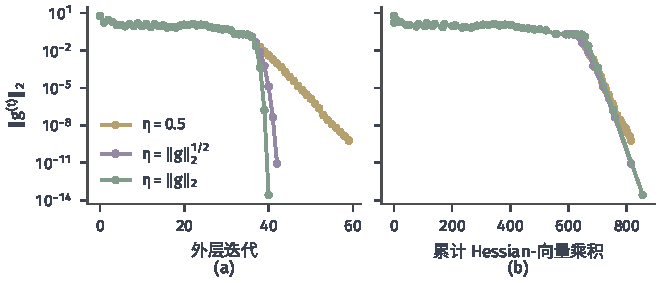
\includegraphics[width=112.0mm]{figures/05-optimization/06-constrained-optimization/matplotlib/mfo-inexact-newton/figure.pdf}
 \caption{$n=500$，$\bm{A}$的特征值在$1$到$100$之间等距，随机起点固定，球面上的Newton--CG加回溯线搜索。内层容差分别取$\eta=0.5$（黄）、$\min\{0.5,\lVert\bm{g}\rVert_2^{1/2}\}$（紫）、$\min\{0.5,\lVert\bm{g}\rVert_2\}$（绿）。(a)~按外层迭代。(b)~按累计Hessian--向量乘积。}
 \label{fig:mfo-inexact-newton}
\end{BookInlineFigure}

\paragraph{负曲率与切向数值误差}
内层CG计算$\langle\bm{d},\bm{H}[\bm{d}]\rangle$时，若它不大于零，说明遇到了负曲率方向，线性方程的解不再是模型的极小点。这时要停止CG：若是第一步，取负梯度方向；否则返回当前的$\bm{v}$，它仍是下降方向。

另一个要小心的是舍入误差。理论上$\bm{H}$把切空间映到切空间，CG的向量始终是切向的。实际计算中会累积沿法向的分量，维数高、CG步数多时尤其明显。常用做法是每隔若干步把$\bm{v}$、$\bm{r}$和$\bm{d}$重新投影到切空间。


\section{拟Newton法}
\label{sec:mfo-quasi-newton}

Hessian难以形成或求解时，第~\ref{chap:quasi-newton}章用相邻两点的梯度差逐步学习曲率。流形上的困难在于，步、梯度差和曲率近似分属不同的切空间。这就需要回答：怎样把这些量放到同一切空间中，使割线关系和正定性仍然成立？

\subsection{黎曼BFGS}
\label{sec:mfo-rbfgs}

\paragraph{主要思想}
割线关系需要一个步和一个梯度差。把它们都放到新点$\bm{x}^{+}=R_{\bm{x}}(\alpha\bm{d})$的切空间：
\begin{equation}
 \bm{s}=\mathcal{T}_{\bm{x}\to\bm{x}^{+}}(\alpha\bm{d}),\qquad
 \bm{y}=\bm{g}^{+}-\mathcal{T}_{\bm{x}\to\bm{x}^{+}}(\bm{g}).
 \label{eq:mfo-curvature-pair}
\end{equation}
这样$\bm{s},\bm{y}\in T_{\bm{x}^{+}}M$，内积用该点的度量计算。

旧的近似算子$\bm{B}$作用在$T_{\bm{x}}M$上，也要搬过去。自然的办法如图~\ref{fig:mfo-operator-square}所示，先搬回旧切空间，作用$\bm{B}$，再搬到新切空间：
\begin{equation}
 \widetilde{\bm{B}}=\mathcal{T}\,\bm{B}\,\mathcal{T}^{-1}.
 \label{eq:mfo-operator-transport}
\end{equation}

\begin{BookInlineFigure}
 \centering
 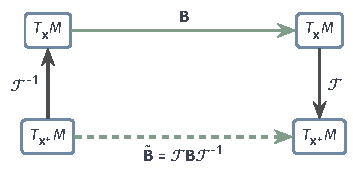
\includegraphics[width=59.8mm]{figures/05-optimization/06-constrained-optimization/tikz/mfo-operator-square/figure.pdf}
 \caption{曲率算子的搬运。绿色实线是旧切空间上的算子，虚线是新切空间上的算子，它由另外三段复合而成：先用$\mathcal{T}^{-1}$回到旧切空间，作用$\bm{B}$，再用$\mathcal{T}$搬到新切空间。}
 \label{fig:mfo-operator-square}
\end{BookInlineFigure}

这个构造对$\mathcal{T}$有要求。若$\mathcal{T}$等距，则$\widetilde{\bm{B}}$仍是自伴的，正定性也保留，因为
\[
 \langle\bm{u},\widetilde{\bm{B}}\bm{u}\rangle=\langle\mathcal{T}^{-1}\bm{u},\bm{B}\mathcal{T}^{-1}\bm{u}\rangle.
\]

等距这一条不能省略。在标准正交坐标下取$\mathcal{T}=\operatorname{diag}(1,\tfrac12)$，这是一个把第二个方向缩短的非等距映射。取对称正定的$\bm{B}$，计算得到
\[
 \bm{B}=\begin{bmatrix}2&1\\1&2\end{bmatrix},\qquad
 \mathcal{T}\bm{B}\mathcal{T}^{-1}=\begin{bmatrix}2&2\\\tfrac12&2\end{bmatrix},
\]
这个矩阵已经不对称了。所以投影搬运不能照搬式~\eqref{eq:mfo-operator-transport}，通常要改用等距搬运，或在搬运后作自伴化处理。

在$T_{\bm{x}^{+}}M$上做欧氏BFGS公式的类比，\term{黎曼BFGS}（Riemannian BFGS）的更新是
\begin{equation}
 \bm{B}^{+}[\bm{u}]=\widetilde{\bm{B}}[\bm{u}]-\frac{\langle\widetilde{\bm{B}}\bm{s},\bm{u}\rangle}{\langle\bm{s},\widetilde{\bm{B}}\bm{s}\rangle}\widetilde{\bm{B}}\bm{s}+\frac{\langle\bm{y},\bm{u}\rangle}{\langle\bm{y},\bm{s}\rangle}\bm{y}.
 \label{eq:mfo-rbfgs}
\end{equation}

代入$\bm{u}=\bm{s}$，前两项抵消，第三项给出$\bm{B}^{+}[\bm{s}]=\bm{y}$，这是新切空间内的割线关系。

记$\bm{W}$为$\bm{B}$的逆，$\rho=1/\langle\bm{s},\bm{y}\rangle$。在等距搬运下，用第~\ref{chap:quasi-newton}章的做法可得逆形式，它能直接给出方向$\bm{d}=-\bm{W}\bm{g}$，不必解方程：
\begin{equation}
 \bm{W}^{+}[\bm{u}]=\bm{V}^{*}\widetilde{\bm{W}}\bm{V}[\bm{u}]+\rho\langle\bm{s},\bm{u}\rangle\bm{s},\qquad
 \bm{V}[\bm{u}]=\bm{u}-\rho\langle\bm{s},\bm{u}\rangle\bm{y},
 \label{eq:mfo-rbfgs-inverse}
\end{equation}
其中$\bm{V}^{*}$是$\bm{V}$关于度量的伴随算子：
\[
 \bm{V}^{*}[\bm{u}]=\bm{u}-\rho\langle\bm{y},\bm{u}\rangle\bm{s}.
\]

\paragraph{曲率条件}
要使$\bm{B}^{+}$保持正定，需要$\langle\bm{s},\bm{y}\rangle>0$。欧氏情形由Wolfe条件保证，流形上要重新核对。设$\mathcal{T}$等距，由式~\eqref{eq:mfo-curvature-pair}，
\[
 \langle\bm{s},\bm{y}\rangle=\alpha\langle\mathcal{T}\bm{d},\bm{g}^{+}\rangle-\alpha\langle\bm{d},\bm{g}\rangle.
\]

Wolfe条件控制的量是沿回缩曲线的导数，记回缩曲线在新点的速度为$\mathcal{T}^{\mathrm{D}}\bm{d}$：
\[
 \langle\bm{g}^{+},\mathcal{T}^{\mathrm{D}}\bm{d}\rangle\geq c_2\langle\bm{g},\bm{d}\rangle.
\]
这和上一式的$\langle\mathcal{T}\bm{d},\bm{g}^{+}\rangle$是不同的量。两者若只差一个正因子$b$，即
\[
 \mathcal{T}\bm{d}=b\,\mathcal{T}^{\mathrm{D}}\bm{d},
\]
代入就有
\begin{equation}
 \langle\bm{s},\bm{y}\rangle\geq\alpha(bc_2-1)\langle\bm{g},\bm{d}\rangle.
 \label{eq:mfo-locking}
\end{equation}
下降方向满足$\langle\bm{g},\bm{d}\rangle<0$，所以$bc_2<1$时右端为正。

球面上用平行移动沿大圆走，方向恰好与回缩曲线同向。第~\ref{sec:mfo-transport}节的微分回缩长度是$\lVert\bm{d}\rVert_2/r^2$，平行移动保持长度，所以$b=r^2=1+\alpha^2\lVert\bm{d}\rVert_2^2$。贯穿例第$0$轮$\alpha=\tfrac12$，$b=\tfrac{98}{81}\approx1.21$，只要$c_2<0.826$就满足。

不满足上述配套关系时，曲率条件没有保证，要在运行中检查：若$\langle\bm{s},\bm{y}\rangle$不够大，就跳过这一次更新，只保留搬运后的$\widetilde{\bm{W}}$。

\needspace{6\baselineskip}
\paragraph{变量}
\begin{itemize}
 \item $\bm{x}^{(t)}$：当前点；$\bm{g}^{(t)}$：黎曼梯度，存它在切空间基下的二维坐标。
 \item $(\bm{E}_1^{(t)},\bm{E}_2^{(t)})$：切空间的标准正交基，用平行移动从上一轮搬来。
 \item $\bm{W}^{(t)}$：逆曲率近似，$2\times2$对称正定矩阵。
 \item $\bm{s},\bm{y}$：曲率对的二维坐标；$\rho=1/\langle\bm{s},\bm{y}\rangle$。
\end{itemize}

因为基是用平行移动搬过来的，向量的搬运在坐标上什么也不用做，式~\eqref{eq:mfo-operator-transport}也变成矩阵不变。这是采用等距搬运的计算便利。

\paragraph{初始化}
取$\bm{W}^{(0)}=\bm{I}_2$，基取$\bm{E}_1,\bm{E}_2$。例中起点是$\bm{x}^{(0)}=\tfrac13(2,2,1)^\top$，$\bm{g}^{(0)}$的坐标是$(\tfrac29,-\tfrac89)^\top$。

\needspace{6\baselineskip}
\paragraph{每轮更新}
\begin{enumerate}
 \item 算方向的坐标$\bm{d}^{(t)}=-\bm{W}^{(t)}\bm{g}^{(t)}$。例中第$0$轮是$(-\tfrac29,\tfrac89)^\top$，与梯度下降相同。

 \item 沿回缩线搜索得到$\alpha^{(t)}$，回缩得到$\bm{x}^{(t+1)}$。例中$\alpha=\tfrac12$，$\bm{x}^{(1)}$与第~\ref{sec:mfo-rgd}节相同。

 \item 用式~\eqref{eq:mfo-parallel-transport}搬运基，并算新梯度的坐标。例中
 \[
  \bm{g}^{(1)}\approx(-0.3938,\ -0.2433)^\top.
 \]

 \item 由式~\eqref{eq:mfo-curvature-pair}算曲率对。平行移动下坐标不变，例中
 \[
  \begin{gathered}
  \bm{s}=\frac12\bm{d}^{(0)}\approx(-0.1111,\ 0.4444)^\top,\\
  \bm{y}=\bm{g}^{(1)}-\bm{g}^{(0)}\approx(-0.6160,\ 0.6456)^\top.
  \end{gathered}
 \]

 \item 检查曲率。例中$\langle\bm{s},\bm{y}\rangle\approx0.3554>0$，可以更新，$\rho\approx2.8139$。

 \item 由式~\eqref{eq:mfo-rbfgs-inverse}更新$\bm{W}$。例中
 \[
  \bm{W}^{(1)}\approx\begin{bmatrix}0.7274&0.5219\\0.5219&1.1864\end{bmatrix}.
 \]
\end{enumerate}

第$1$轮方向的坐标是
\[
 \bm{d}^{(1)}=-\bm{W}^{(1)}\bm{g}^{(1)}\approx(0.4134,\ 0.4941)^\top,
\]
方向导数约为$-0.2830$，下降。试探$\alpha=1$得到
\[
 \bm{x}^{(2)}\approx(0.9955,-0.0010,-0.0944)^\top,\qquad f\approx0.5134,\qquad\lVert\bm{g}^{(2)}\rVert_2\approx0.2819.
\]

下面对照$\bm{x}^{(1)}$处真实的黎曼Hessian与$\bm{B}^{(1)}=(\bm{W}^{(1)})^{-1}$的坐标：
\[
 \bm{H}^{(1)}\approx\begin{bmatrix}1.47&-1.14\\-1.14&1.65\end{bmatrix},\qquad
 \bm{B}^{(1)}\approx\begin{bmatrix}2.01&-0.88\\-0.88&1.23\end{bmatrix}.
\]

只做一次更新，曲率对只在$\bm{s}$方向上提供信息，整个矩阵还不准确，割线方向上$\bm{B}^{(1)}\bm{s}=\bm{y}$精确成立。当$\lVert\bm{g}^{(t)}\rVert_2\leq10^{-6}$时结束，最终得到$\bm{x}^{(T)}\approx\pm\bm{e}_1$。

\paragraph{保证的来源}
下降性来自$\bm{W}$的正定性，而正定性要有三个条件同时成立：正定初值、保持自伴性和内积的搬运、每轮$\langle\bm{s},\bm{y}\rangle>0$。线搜索和回缩若不满足前述配套，后者就必须靠运行中检查来维持。

局部超线性收敛的结论针对具体的算法版本。已有的分析通常假定等距搬运、Wolfe型线搜索，以及类似式~\eqref{eq:mfo-locking}的配套条件；证明需要处理搬运带来的额外误差项，篇幅较长，读者可查阅黎曼拟Newton方法的专门文献。使用投影搬运、Armijo线搜索的简化版本在实际中也常常有效，但这些保证不能直接移用。

\subsection{有限记忆方法}
\label{sec:mfo-lbfgs}

\paragraph{主要思想}
稠密的$\bm{W}$要占$O(n^2)$存储，且每轮都要搬运一个算子。第~\ref{chap:quasi-newton}章的L-BFGS只保留最近$m$对$(\bm{s},\bm{y})$，用两层递推算出$\bm{W}\bm{g}$，流形上的版本思路相同，只是这些向量要跟着当前点走。

每次迭代后，把所存的向量对都搬到新切空间。递推仍是第~\ref{chap:quasi-newton}章的式子，内积换成当前点的度量。第一层从最新一对到最旧一对，初始$\bm{q}=\bm{g}$：
\begin{equation}
 \xi_j=\rho_j\langle\bm{s}_j,\bm{q}\rangle,\qquad
 \bm{q}\leftarrow\bm{q}-\xi_j\bm{y}_j.
 \label{eq:mfo-lbfgs-loop1}
\end{equation}

中间取$\bm{z}=\gamma\bm{q}$，尺度用最新的一对计算：
\[
 \gamma=\frac{\langle\bm{s},\bm{y}\rangle}{\langle\bm{y},\bm{y}\rangle}.
\]

第二层从最旧一对到最新一对：
\begin{equation}
 \eta_j=\rho_j\langle\bm{y}_j,\bm{z}\rangle,\qquad
 \bm{z}\leftarrow\bm{z}+(\xi_j-\eta_j)\bm{s}_j.
 \label{eq:mfo-lbfgs-loop2}
\end{equation}
最后的搜索方向是$\bm{d}=-\bm{z}$。

用$m=1$在贯穿例的第$1$轮算一遍，曲率对取上一小节的结果。第一层给出
\[
 \xi\approx-0.1811,\qquad\bm{q}\approx(-0.5053,\ -0.1263)^\top.
\]

中间$\gamma\approx0.4463$，所以$\bm{z}\approx(-0.2255,-0.0564)^\top$。第二层$\eta\approx0.2885$，于是
\[
 \bm{z}\approx(-0.1734,\ -0.2651)^\top,\qquad\bm{d}\approx(0.1734,\ 0.2651)^\top.
\]
方向导数约为$-0.1328$，是下降方向。它与完整BFGS的$(0.4134,0.4941)^\top$方向相近、长度不同，因为初始尺度从$\bm{I}$换成了$\gamma\bm{I}$。

\paragraph{历史长度与成本}
增大$m$减少迭代数，但每轮要搬运和内积的向量也增多。图~\ref{fig:mfo-lbfgs-memory}是$n=500$的实验，$m$从$1$增加到$50$，迭代数从$268$降到$141$，降幅不到一半，而按每轮$(3+10m)$次向量运算的粗略模型，总运算量却增加了约$20$倍。

\begin{BookInlineFigure}
 \centering
 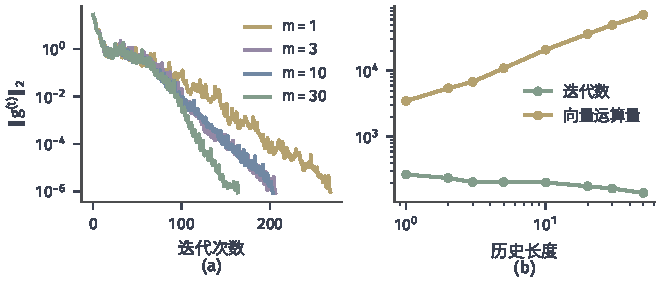
\includegraphics[width=112.0mm]{figures/05-optimization/06-constrained-optimization/matplotlib/mfo-lbfgs-memory/figure.pdf}
 \caption{$n=500$，$\bm{A}$的特征值在$1$到$100$之间等距，随机起点固定，使用平行移动的有限记忆黎曼BFGS，容差$\lVert\bm{g}\rVert_2\leq10^{-6}$。(a)~不同历史长度$m$的梯度范数。(b)~达到容差的迭代数（绿）和按每轮$3+10m$次向量运算估算的总运算量（黄）。}
 \label{fig:mfo-lbfgs-memory}
\end{BookInlineFigure}

这个实验中$\bm{A}$是对角阵，乘一次很便宜，搬运的代价显得突出。若$\bm{A}$乘向量很昂贵，或回缩的代价高，向量运算占比就小，较大的$m$更合算。

历史信息被截断后，完整BFGS的局部结论不再自动成立。有限记忆方法的曲率近似只包含$m$个方向，一般只有线性收敛的保证，这与欧氏情形一致。此外，为降低成本，一些实现只在需要时才搬运向量，这也属于另一种算法版本，其性质要另行核对。

\section{黎曼信赖域}
\label{sec:mfo-trust-region}

第~\ref{sec:mfo-newton}节的起点上，Newton步是上升方向；第~\ref{sec:mfo-pullback}节的$s=1$处，模型误差已经达到$\tfrac{5}{18}$。这两件事都说明，曲率模型只在有限的尺度内可信。第~\ref{chap:trust-region}章的信赖域正是处理这个问题的，本节回答它怎样搬到切空间上，又有哪些新的条件要核对。

\paragraph{主要思想}
在当前切空间的有限半径内近似最小化模型~\eqref{eq:mfo-model}：
\begin{equation}
 \min_{\bm{v}\in T_{\bm{x}}M}\ m_{\bm{x}}(\bm{v})\quad\text{s.t.}\quad\lVert\bm{v}\rVert_2\leq\Delta.
 \label{eq:mfo-rtr-subproblem}
\end{equation}
半径$\Delta$在切空间里度量，子问题是线性空间上的普通信赖域子问题。

得到候选步$\bm{v}$后，回缩到流形上，比较实际下降与预测下降：
\begin{equation}
 \rho=\frac{f(\bm{x})-f(R_{\bm{x}}(\bm{v}))}{m_{\bm{x}}(\bm{0})-m_{\bm{x}}(\bm{v})}.
 \label{eq:mfo-rtr-ratio}
\end{equation}
分子必须用回缩后的点，所以回缩造成的偏差也一并得到了检验。

接受和半径的规则沿用第~\ref{chap:trust-region}章：$\rho\geq\tfrac14$时接受，否则留在原地；$\rho<\tfrac14$时半径缩小为$\tfrac14$倍，$\rho\geq\tfrac34$且步到达边界时半径加倍（不超过上限$\Delta_{\max}$），其余情形半径不变。这样曲率模型只在获得检验的尺度内被使用。这就是\term{黎曼信赖域}（Riemannian trust region）方法。

图~\ref{fig:mfo-rtr-disc}画出贯穿例第$0$轮的几何。紫色椭圆是切平面上半径为$1$的圆盘，它的回缩像是球面上的绿色小圆。候选步在切平面上产生，回缩后落在绿圈之内或之上。

\begin{BookInlineFigure}
 \centering
 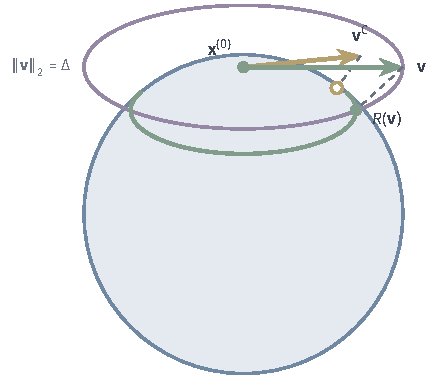
\includegraphics[width=74.0mm]{figures/05-optimization/06-constrained-optimization/tikz/mfo-rtr-disc/figure.pdf}
 \caption{切平面上的信赖域及其回缩像。紫色是切平面上半径$\Delta=1$的圆的边界，绿色闭曲线是它在归一化回缩下的像。黄箭头是Cauchy步$\bm{v}^{\mathrm{C}}$，绿箭头是截断CG得到的步$\bm{v}$，虚线是回缩，实心点是接受的新点。}
 \label{fig:mfo-rtr-disc}
\end{BookInlineFigure}

\subsection{子问题的求解}
\label{sec:mfo-rtr-subproblem}

\paragraph{Cauchy步}
最便宜的办法是沿负梯度在半径内最小化模型，这就是第~\ref{chap:trust-region}章的\term{Cauchy步}（Cauchy step）。记沿负梯度的曲率为
\[
 \kappa=\frac{\langle\bm{g},\bm{H}\bm{g}\rangle}{\lVert\bm{g}\rVert_2^2},
\]
当$\kappa>0$且$\lVert\bm{g}\rVert_2/\kappa<\Delta$时取$\bm{v}^{\mathrm{C}}=-\bm{g}/\kappa$，否则走到边界。

第~\ref{chap:trust-region}章证明了它的预测下降满足下面的下限，切空间上的证明一字不改：
\begin{equation}
 m(\bm{0})-m(\bm{v}^{\mathrm{C}})\geq\frac12\lVert\bm{g}\rVert_2\min\Bigl\{\Delta,\ \frac{\lVert\bm{g}\rVert_2}{\lVert\bm{H}\rVert_2}\Bigr\}.
 \label{eq:mfo-cauchy-decrease}
\end{equation}

\paragraph{截断共轭梯度}
只用Cauchy步相当于梯度法，为了利用曲率，用第~\ref{chap:trust-region}章的\term{截断共轭梯度法}（truncated conjugate gradient）在切空间内迭代。迭代从$\bm{v}=\bm{0}$开始，第一步就是Cauchy步的方向，之后模型值单调下降，所以最终的预测下降不低于Cauchy步。

三种情形下停止：残差足够小；遇到负曲率时沿当前方向走到边界；下一步要越界时截断在边界。残差容差取
\begin{equation}
 \lVert\bm{r}\rVert_2\leq\lVert\bm{r}_0\rVert_2\min\bigl\{\lVert\bm{r}_0\rVert_2^{\theta},\ \varkappa\bigr\},
 \label{eq:mfo-rtr-forcing}
\end{equation}
其中$\theta>0$，$\varkappa\in(0,1)$。

\needspace{6\baselineskip}
\paragraph{变量}
\begin{itemize}
 \item $\bm{x}^{(t)}$：当前点；$\Delta^{(t)}$：半径；$\bm{g},\bm{H}$：当前切空间基下的梯度坐标和Hessian。
 \item $\bm{v}_j$：内层的当前步，$\bm{r}_j$：残差$\bm{H}\bm{v}_j+\bm{g}$，$\bm{p}_j$：共轭方向，均为二维坐标。
 \item 参数：$\theta=1$，$\varkappa=0.1$。
\end{itemize}

\paragraph{初始化}
例中$\bm{x}^{(0)}=\tfrac13(2,2,1)^\top$，$\Delta^{(0)}=1$。由第~\ref{sec:mfo-newton}节的数据，
\[
 \bm{g}=\begin{bmatrix}2/9\\-8/9\end{bmatrix},\qquad
 \bm{H}=\begin{bmatrix}1&-10/9\\-10/9&2/3\end{bmatrix}.
\]
内层初始化为$\bm{v}_0=\bm{0}$，$\bm{r}_0=\bm{g}$，$\bm{p}_0=-\bm{g}$。

\needspace{6\baselineskip}
\paragraph{每轮更新}
\begin{enumerate}
 \item 计算$\kappa_j=\langle\bm{p}_j,\bm{H}\bm{p}_j\rangle$。例中第$0$步$\bm{H}\bm{p}_0\approx(-1.2099,0.8395)^\top$，$\kappa_0\approx1.0151>0$。

 \item 若$\kappa_j\leq0$，沿$\bm{p}_j$走到边界后结束内层。否则取$\alpha_j=\lVert\bm{r}_j\rVert_2^2/\kappa_j$，并算$\bm{v}_{j+1}=\bm{v}_j+\alpha_j\bm{p}_j$。例中$\alpha_0=\tfrac{153}{185}\approx0.8270$，
 \[
  \bm{v}_1=\Bigl(-\frac{34}{185},\ \frac{136}{185}\Bigr)^\top\approx(-0.1838,\ 0.7351)^\top.
 \]
 它的长度约为$0.7578<1$，不越界，这就是Cauchy步，预测下降$0.3471$。

 \item 更新残差和方向：
 \[
  \begin{gathered}
  \bm{r}_{j+1}=\bm{r}_j+\alpha_j\bm{H}\bm{p}_j,\qquad
  \beta_j=\frac{\lVert\bm{r}_{j+1}\rVert_2^2}{\lVert\bm{r}_j\rVert_2^2},\\
  \bm{p}_{j+1}=-\bm{r}_{j+1}+\beta_j\bm{p}_j.
  \end{gathered}
 \]
 例中
 \[
  \bm{r}_1\approx(-0.7784,\ -0.1946)^\top,\quad\beta_0\approx0.7668,\quad\bm{p}_1\approx(0.6080,\ 0.8762)^\top.
 \]

 \item 例中第$1$步$\kappa_1\approx-0.302<0$，遇到负曲率。解$\lVert\bm{v}_1+\tau\bm{p}_1\rVert_2=1$，得$\tau\approx0.3023$，于是
 \[
  \bm{v}=\bm{v}_1+\tau\bm{p}_1=(0,\ 1)^\top.
 \]
 所以$\bm{v}=\bm{E}_2$，正好是切空间的基向量，内层结束。

 \item 算预测下降。例中$m(\bm{v})-f(\bm{x})=-\tfrac89+\tfrac13$，所以预测下降$\tfrac59$。

 \item 回缩并算$\rho$。例中$\bm{x}^{(0)}+\bm{E}_2=\tfrac13(4,1,-1)^\top$，长度$\sqrt2$，
 \[
  R_{\bm{x}^{(0)}}(\bm{v})=\frac{(4,1,-1)^\top}{3\sqrt2}\approx(0.9428,0.2357,-0.2357)^\top,\qquad f=\frac{11}{18}.
 \]
 实际下降$\tfrac89-\tfrac{11}{18}=\tfrac{5}{18}$，由式~\eqref{eq:mfo-rtr-ratio}得$\rho=\tfrac12$。

 \item 按规则更新。例中$\rho=\tfrac12\in[\tfrac14,\tfrac34)$，接受这一步，半径保持$1$。
\end{enumerate}

对比只用Cauchy步：其回缩点的目标值是$0.6684$，$\rho\approx0.635$，实际下降$0.2205$；截断CG多用一次Hessian--向量乘积，实际下降增加到$0.2778$。负曲率方向在这里提供了额外的下降，而第~\ref{sec:mfo-newton}节的Newton方向恰恰是上升的。

图~\ref{fig:mfo-rtr-model}把这一轮放回切平面坐标。在原点附近模型与拉回的等值线几乎重合，到半径$1$的边界上两者已明显不同。

\begin{BookInlineFigure}
 \centering
 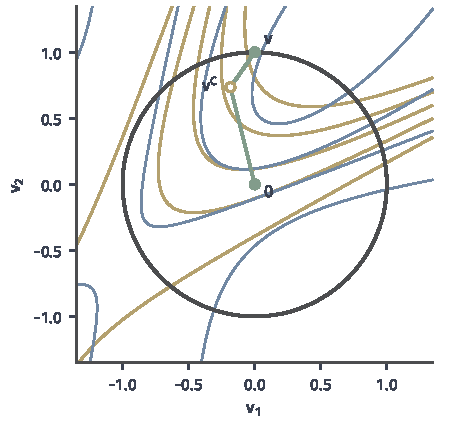
\includegraphics[width=78.0mm]{figures/05-optimization/06-constrained-optimization/matplotlib/mfo-rtr-model/figure.pdf}
 \caption{$\bm{x}^{(0)}$处切平面坐标下的模型（黄）与拉回目标（蓝）的等值线，两组曲线使用相同的水平。深灰圆是半径$\Delta=1$的边界，绿色折线是截断CG的路径，空心点是Cauchy步。模型不定，等值线不闭合。}
 \label{fig:mfo-rtr-model}
\end{BookInlineFigure}

后面几轮的结果如表~\ref{tab:mfo-rtr-run}。第$1$轮起都在内部收敛，$\rho$迅速接近一，模型变得可信，与Newton法的快速局部收敛衔接。第$4$轮$\lVert\bm{g}\rVert_2$约为$9.4\times10^{-11}$，低于容差，迭代结束，最终得到$\bm{x}^{(4)}\approx\bm{e}_1$。

\begin{BookInlineTable}
 \centering
 \caption{贯穿例的黎曼信赖域，$\Delta^{(0)}=1$。}
 \label{tab:mfo-rtr-run}
 \begin{tabular}{llllll}
  \toprule
  $t$ & $f(\bm{x}^{(t)})$ & $\lVert\bm{g}^{(t)}\rVert_2$ & 内层结束方式 & 预测下降 & $\rho$\\
  \midrule
  $0$ & $0.8889$ & $0.9162$ & 负曲率 & $0.5556$ & $0.500$\\
  $1$ & $0.6111$ & $0.7115$ & 残差 & $0.1279$ & $0.844$\\
  $2$ & $0.5031$ & $0.0928$ & 残差 & $3.15\times10^{-3}$ & $0.994$\\
  $3$ & $0.5000$ & $4.68\times10^{-4}$ & 残差 & $1.04\times10^{-7}$ & $1.000$\\
  \bottomrule
 \end{tabular}
\end{BookInlineTable}

\paragraph{进展条件}
实际运行中要求候选步的模型下降至少达到Cauchy步的某个比例，这是全局收敛分析的常用条件：存在$c\in(0,\tfrac12]$，使得
\begin{equation}
 m(\bm{0})-m(\bm{v})\geq c\lVert\bm{g}\rVert_2\min\Bigl\{\Delta,\ \frac{\lVert\bm{g}\rVert_2}{\beta}\Bigr\},
 \label{eq:mfo-cauchy-fraction}
\end{equation}
这里$\beta\geq\lVert\bm{H}\rVert_2$。截断CG自动满足它，取$c=\tfrac12$。

这个条件只针对一阶进展。更强的二阶驻点保证要求子问题求解器能处理负曲率。截断CG从$\bm{v}=\bm{0}$出发，第一步方向是$-\bm{g}$，当$\bm{g}=\bm{0}$时立即停止。贯穿例中恰好落在鞍点$\bm{e}_2$时，$\bm{g}=\bm{0}$，切向曲率有$-1$，但截断CG返回零步，迭代就此停住。

要逃出这样的点，须在小梯度时计算$\bm{H}$的最小特征值及其特征向量，并沿该方向走一步，这个步称为特征步。第~\ref{chap:saddle-points}章的讨论在切空间上同样适用。

\subsection{模型与回缩条件}
\label{sec:mfo-rtr-conditions}

\paragraph{近似误差进入比值}
由式~\eqref{eq:mfo-rtr-ratio}，因为$m(\bm{0})=f(\bm{x})$，比值的偏差可以写成
\begin{equation}
 1-\rho=\frac{\hat{f}_{\bm{x}}(\bm{v})-m_{\bm{x}}(\bm{v})}{m_{\bm{x}}(\bm{0})-m_{\bm{x}}(\bm{v})}.
 \label{eq:mfo-rho-gap}
\end{equation}
分子是拉回目标与模型的差，分母是预测下降，所有误差都集中在分子。分子由三部分组成：回缩对一阶和二阶信息的近似、$\bm{H}$与真实曲率的差、拉回函数的高阶余项。

分母受子问题求解精度的影响。子问题解得差，分母偏小，比值波动就大。所以这个比值同时检验了模型、回缩和子问题三者。

\paragraph{达到小梯度}
下面的定理说明，什么样的近似误差足以保证梯度变小。这里假定拉回目标与模型之差被二次函数界住。

\begin{theorem}[黎曼信赖域的迭代界]
 \label{thm:mfo-rtr-complexity}
 设$f$有下界$f^\star$，所有迭代满足式~\eqref{eq:mfo-cauchy-fraction}，$\lVert\bm{H}^{(t)}\rVert_2\leq\beta$，并且存在$C\geq\beta$，使
 \begin{equation}
  \bigl\lvert\hat{f}_{\bm{x}^{(t)}}(\bm{v})-m_{\bm{x}^{(t)}}(\bm{v})\bigr\rvert\leq\frac C2\lVert\bm{v}\rVert_2^2,\qquad\lVert\bm{v}\rVert_2\leq\Delta_{\max}.
  \label{eq:mfo-model-error}
 \end{equation}
 按本节规则更新半径。若前$T$轮都有$\lVert\bm{g}^{(t)}\rVert_2\geq\varepsilon$，令
 \begin{equation}
  \underline{\Delta}=\min\Bigl\{\Delta^{(0)},\ \frac{c\varepsilon}{8C}\Bigr\},
  \label{eq:mfo-rtr-radius-floor}
 \end{equation}
 则
 \begin{equation}
  T\leq\frac{6\bigl(f(\bm{x}^{(0)})-f^\star\bigr)}{c\,\varepsilon\,\underline{\Delta}}+\frac12\log_2\frac{\Delta^{(0)}}{\underline{\Delta}}.
  \label{eq:mfo-rtr-complexity}
 \end{equation}
 所以小的$\varepsilon$对应的迭代次数为$O(1/\varepsilon^2)$。
\end{theorem}

\begin{proof}
 第一步证明半径小时比值接近一。设$\lVert\bm{g}\rVert_2\geq\varepsilon$，并设$\Delta\leq c\varepsilon/(2C)$。因为$c\leq\tfrac12$，$C\geq\beta$，所以$\Delta$不超过$\lVert\bm{g}\rVert_2/\beta$，式~\eqref{eq:mfo-cauchy-fraction}给出预测下降至少为$c\varepsilon\Delta$。

 再由式~\eqref{eq:mfo-rho-gap}和式~\eqref{eq:mfo-model-error}，并用$\lVert\bm{v}\rVert_2\leq\Delta$，得到
 \[
  \lvert1-\rho\rvert\leq\frac{C\Delta^2/2}{c\varepsilon\Delta}=\frac{C\Delta}{2c\varepsilon}\leq\frac14.
 \]
 于是$\rho\geq\tfrac34$，半径不会缩小。

 第二步给出半径的下界。半径只在$\rho<\tfrac14$时缩小，此时一定有$\Delta>c\varepsilon/(2C)$，缩小后仍大于$c\varepsilon/(8C)$。因此所有轮都有$\Delta^{(t)}\geq\underline{\Delta}$。

 第三步数接受的轮数$T_{\mathrm{a}}$。接受时$\rho\geq\tfrac14$，再用预测下降的下限，并用$\underline{\Delta}\leq\varepsilon/\beta$，得到
 \[
  f(\bm{x}^{(t)})-f(\bm{x}^{(t+1)})\geq\frac14c\varepsilon\underline{\Delta}.
 \]
 目标总下降量不超过$f(\bm{x}^{(0)})-f^\star$，所以
 \[
  T_{\mathrm{a}}\leq\frac{4\bigl(f(\bm{x}^{(0)})-f^\star\bigr)}{c\varepsilon\underline{\Delta}}.
 \]

 第四步数拒绝的轮数$T_{\mathrm{r}}$。每次拒绝半径乘$\tfrac14$，每次接受半径至多乘$2$，所以
 \[
  \underline{\Delta}\leq\Delta^{(T)}\leq\Delta^{(0)}\,2^{T_{\mathrm{a}}}\,4^{-T_{\mathrm{r}}}.
 \]
 取对数得
 \[
  T_{\mathrm{r}}\leq\frac12T_{\mathrm{a}}+\frac12\log_2\frac{\Delta^{(0)}}{\underline{\Delta}}.
 \]

 把$T=T_{\mathrm{a}}+T_{\mathrm{r}}$合起来，就得到式~\eqref{eq:mfo-rtr-complexity}。
\end{proof}

定理的假设分三项，各起一种作用。式~\eqref{eq:mfo-cauchy-fraction}保证分母足够大；$\lVert\bm{H}\rVert_2\leq\beta$保证小半径时走到边界的量级被正确估计；式~\eqref{eq:mfo-model-error}保证分子足够小。

这个假设对回缩的要求不高。把式~\eqref{eq:mfo-pullback-smooth}类型的双侧上界与$\lVert\bm{H}\rVert_2\leq\beta$相加，就得到式~\eqref{eq:mfo-model-error}，这时$\bm{H}$甚至不必是真实的Hessian，例如用$\bm{H}=\bm{0}$也行，此时算法退化为带半径控制的梯度法。在紧流形上，光滑目标和光滑回缩自动满足该假设。

\paragraph{二阶驻点与快速局部收敛}
定理只说梯度变小。要达到近似二阶驻点，即$\bm{H}\succeq-\varepsilon_H\bm{I}$，需要额外条件：$\bm{H}$在拉回Hessian的一定精度内，模型误差有三次界，子问题在负曲率时能产生下降正比于负曲率立方的步。在这些条件下，迭代次数的量级为$O(\max\{\varepsilon^{-2}\varepsilon_H^{-1},\varepsilon_H^{-3}\})$，证明沿用定理~\ref{thm:mfo-rtr-complexity}的结构并加入负曲率情形，读者可查阅\scite{math-boumal2023optimization}。

即使达到了二阶驻点，也不能断言是局部极小。第~\ref{sec:mfo-optimality}节的$x_2^3$例子满足二阶必要条件却不是局部极小。近似二阶驻点只是必要条件的数值形式。

快速局部收敛需要模型足够精确。若迭代收敛到非退化的极小点，$\bm{H}^{(t)}$是真实的黎曼Hessian，并用式~\eqref{eq:mfo-rtr-forcing}控制内层精度，那么$\rho\to1$，半径不再起作用，方法变成非精确Newton，局部收敛阶至少是$\min\{1+\theta,2\}$。证明需要回缩与Hessian的局部误差估计，这里只说明机制：第~\ref{sec:mfo-pullback}节的附加项正比于$\lVert\bm{g}\rVert_2$，一般回缩也不破坏这一速度。

图~\ref{fig:mfo-rtr-history}是$n=300$的问题。半径初值$2$过大，第$0$轮$\rho\approx0.20$被拒绝，半径缩小到$0.5$；第$1$轮$\rho\approx0.80$，半径扩大到$1$，此后半径保持不变。最后几轮$\rho\approx1$，梯度范数快速下降。

\begin{BookInlineFigure}
 \centering
 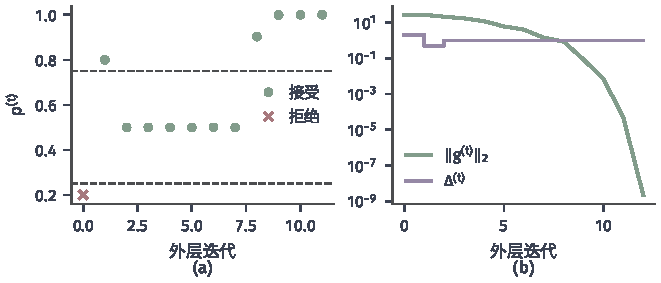
\includegraphics[width=112.0mm]{figures/05-optimization/06-constrained-optimization/matplotlib/mfo-rtr-history/figure.pdf}
 \caption{$n=300$，$\bm{A}$的特征值在$1$到$100$之间等距，随机起点固定，$\theta=1$，$\varkappa=0.1$，$\Delta^{(0)}=2$。(a)~各轮的比值$\rho$，绿点接受，红叉拒绝，两条虚线是$\tfrac14$与$\tfrac34$。(b)~梯度范数（绿）和半径（紫）。}
 \label{fig:mfo-rtr-history}
\end{BookInlineFigure}

\section{表示与计算成本}
\label{sec:mfo-representation}

前面的算法都在给定的表示上运行。这一节要回答两个问题：同一对象有多种矩阵记录时应该怎样处理，流形方法与一般约束方法放在同一标准下比较时结果如何。

\paragraph{同一子空间的多种表示}
最小化$k$个最小特征值之和可以写成
\begin{equation}
 \min_{\bm{X}\in\mathrm{St}(k,n)}\ f(\bm{X})=\frac12\operatorname{tr}\bigl(\bm{X}^\top\bm{A}\bm{X}\bigr).
 \label{eq:mfo-subspace-objective}
\end{equation}
对任意$k\times k$正交矩阵$\bm{Q}$，$f(\bm{X}\bm{Q})=f(\bm{X})$，因为迹对循环置换不变。所以目标只取决于$\bm{X}$的列空间，而不取决于所选的基。图~\ref{fig:mfo-grassmann-fibre}(a)中三组不同的基张成同一个平面，目标值相同。

Stiefel流形上的点与子空间的对应是多对一的。子空间全体构成Grassmann空间$\mathrm{Gr}(k,n)$，它是$\mathrm{St}(k,n)$对右乘正交矩阵的商，维数是$k(n-k)$，比Stiefel流形少$k(k-1)/2$。其光滑结构的建立可参考\BookChapterRef{chap:lie-groups}{卷四第29章“Lie群”}。

\begin{BookInlineFigure}
 \centering
 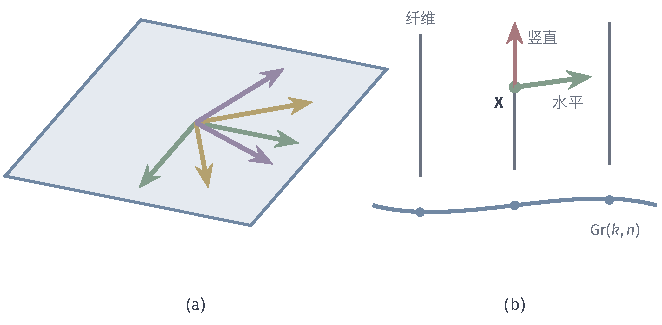
\includegraphics[width=112.0mm]{figures/05-optimization/06-constrained-optimization/tikz/mfo-grassmann-fibre/figure.pdf}
 \caption{子空间的多种表示。(a)~同一平面（浅蓝）的三组标准正交基，绿、黄、紫三组箭头分别对应一种基。(b)~商结构的示意：底部曲线代表$\mathrm{Gr}(k,n)$，每点上方的竖线（纤维）是表示同一子空间的所有$\bm{X}$；红箭头是竖直方向，沿它移动子空间不变，绿箭头是水平方向。}
 \label{fig:mfo-grassmann-fibre}
\end{BookInlineFigure}

\paragraph{竖直方向与水平方向}
沿曲线$\bm{X}\exp(t\bm{\Omega})$（$\bm{\Omega}$反对称）移动，子空间不变，它的速度$\bm{X}\bm{\Omega}$称为竖直方向。与竖直方向正交的切向量满足$\bm{X}^\top\bm{\Delta}=\bm{0}$，它们构成水平空间，每个水平方向都真正改变子空间。

这种分解对梯度有简单的影响。因为$f$沿竖直方向不变，$\operatorname{grad}f$没有竖直分量。由投影公式~\eqref{eq:mfo-stiefel-projection}和$\nabla\bar{f}=\bm{A}\bm{X}$，$\bm{X}^\top\bm{A}\bm{X}$对称，于是
\begin{equation}
 \operatorname{grad}f(\bm{X})=\bm{A}\bm{X}-\bm{X}\bigl(\bm{X}^\top\bm{A}\bm{X}\bigr)=(\bm{I}-\bm{X}\bm{X}^\top)\bm{A}\bm{X}.
 \label{eq:mfo-stiefel-grad}
\end{equation}
满足$\bm{X}^\top\operatorname{grad}f=\bm{0}$，确实是水平的。驻点的条件是$\bm{X}$的列空间是$\bm{A}$的不变子空间。

用贯穿的矩阵算一次。取$\bm{X}=[\bm{x}^{(0)},\bm{E}_1]$，先算
\[
 \bm{X}^\top\bm{A}\bm{X}=\frac19\begin{bmatrix}16&2\\2&25\end{bmatrix},\qquad f(\bm{X})=\frac{41}{18}.
\]

把它代入式~\eqref{eq:mfo-stiefel-grad}，得到
\[
 \operatorname{grad}f(\bm{X})=\frac{1}{27}\begin{bmatrix}-16&-20\\8&10\\16&20\end{bmatrix}.
\]

两列都平行于法向量$\bm{n}=\tfrac13(-2,1,2)^\top$，也就是与平面$\operatorname{span}\bm{X}$垂直的方向。这正好符合水平的要求：要改变一个平面，只能把基朝平面外转动。

取$\alpha=\tfrac12$，先走到$\bm{X}-\tfrac12\operatorname{grad}f(\bm{X})$，然后作回缩。QR回缩与极分解回缩的结果分别是
\[
 \bm{X}^{\mathrm{QR}}\approx\begin{bmatrix}0.8800&0.4504\\0.4738&-0.8549\\0.0338&0.2574\end{bmatrix},\qquad
 \bm{X}^{\mathrm{pol}}\approx\begin{bmatrix}0.8298&0.5373\\0.5580&-0.8025\\0.0076&0.2595\end{bmatrix}.
\]
两者列空间相同，目标值都约为$1.5788$，比原来的$2.2778$小。子空间问题的回缩，只有列空间才有意义，QR分解与极分解的差别不影响目标。

\paragraph{冗余对曲率的影响}
竖直方向对Newton型方法有实质影响。由第~\ref{sec:mfo-optimality}节的做法，Stiefel上的Hessian是
\begin{equation}
 \operatorname{Hess}f(\bm{X})[\bm{\Delta}]=\bm{P}_{\bm{X}}\bigl(\bm{A}\bm{\Delta}-\bm{\Delta}\,\bm{X}^\top\bm{A}\bm{X}\bigr).
 \label{eq:mfo-stiefel-hess}
\end{equation}

取极小点$\bm{X}^\star=[\bm{e}_1,\bm{e}_2]$，此时$\bm{X}^\top\bm{A}\bm{X}$是$\operatorname{diag}(1,2)$，$\mathrm{St}(2,3)$的切空间是$3$维的。取竖直方向$\bm{\Delta}=\bm{X}^\star\bm{\Omega}$，$\bm{\Omega}$是$2\times2$反对称矩阵，代入式~\eqref{eq:mfo-stiefel-hess}算得$\operatorname{Hess}f[\bm{\Delta}]=\bm{0}$，这个方向是零特征方向。

水平方向取$\bm{\Delta}=\bm{e}_3\bm{b}^\top$，算得
\[
 \operatorname{Hess}f[\bm{\Delta}]=\bm{e}_3\,(3b_1,\ 2b_2).
\]
所以$\bm{X}^\star$处Hessian的特征值是$3,2,0$，算子奇异，第~\ref{sec:mfo-newton}节要求的非退化条件在$\mathrm{St}(2,3)$上不成立，而这个零特征值完全是表示引入的。

商结构的办法是把Newton方程限制在水平空间$\bm{X}^\top\bm{\Delta}=\bm{0}$内，这时算子只有$3,2$两个特征值，可逆。实际上就是在$\mathrm{Gr}(k,n)$上计算，但存储仍用矩阵$\bm{X}$。在目标对基变换不变时这样做减少了$k(k-1)/2$个冗余维数。目标若不具备不变性（例如不同列带不同权重），列的次序和基都有意义，就要留在Stiefel流形上。

\paragraph{同一标准下比较}
比较两类方法时，目标、精度和计量单位必须一致，并且要同时报告两个误差。一般约束方法不保证每步可行，只看目标值或只看驻点残差都会误判。下面用问题~\eqref{eq:mfo-subspace-objective}，取$n=200$，$k=5$，$\bm{A}$的特征值在$1$到$100$之间等距。

三种方法都从同一个随机起点出发。黎曼梯度下降和黎曼信赖域使用QR回缩，后者在Grassmann结构上运行。第~\ref{chap:penalty-multiplier-methods}章的增广Lagrange方法用有限记忆拟Newton法解内层问题，迭代中不做回缩。残差统一在当前点作QR所得的$\bm{Q}$上计算，以便不同方法使用同一标准：
\[
 \lVert(\bm{I}-\bm{Q}\bm{Q}^\top)\bm{A}\bm{Q}\rVert_{\mathrm{F}}.
\]

结果见图~\ref{fig:mfo-method-compare}和表~\ref{tab:mfo-method-results}。计量单位是$\bm{A}$乘一列向量的次数。增广Lagrange在迭代中途离开可行集，可行误差最大约为$1.66$，随外层更新才回到机器精度，这时已经用了$10^5$量级的乘积。两种流形方法每一步都保持机器精度的可行性。

\begin{BookInlineFigure}
 \centering
 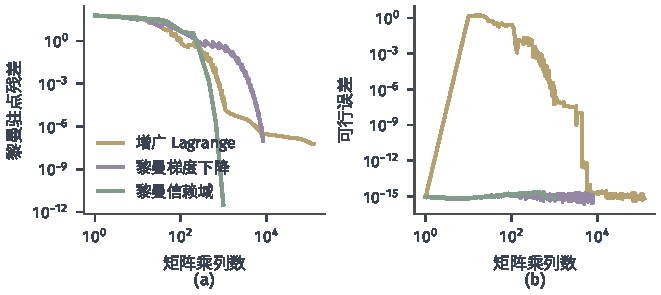
\includegraphics[width=112.0mm]{figures/05-optimization/06-constrained-optimization/matplotlib/mfo-method-compare/figure.pdf}
 \caption{$\mathrm{St}(5,200)$上的子空间问题，横轴是$\bm{A}$乘列向量的累计次数。黄线为增广Lagrange方法，紫线为黎曼梯度下降，绿线为黎曼信赖域。(a)~黎曼驻点残差。(b)~可行误差$\lVert\bm{X}^\top\bm{X}-\bm{I}\rVert_{\mathrm{F}}$。这是单个问题实例的一次运行，三种方法都未作专门调参。}
 \label{fig:mfo-method-compare}
\end{BookInlineFigure}

\begin{BookInlineTable}
 \centering
 \caption{图~\ref{fig:mfo-method-compare}的运行结果，三种方法的黎曼驻点残差的容差均为$10^{-7}$。}
 \label{tab:mfo-method-results}
 \begin{tabular}{lllll}
  \toprule
  方法 & 乘列数 & QR次数 & 驻点残差 & 最大可行误差\\
  \midrule
  增广Lagrange & $123560$ & $0$ & $5.9\times10^{-8}$ & $1.66$\\
  黎曼梯度下降 & $8110$ & $3244$ & $9.9\times10^{-8}$ & $2.4\times10^{-15}$\\
  黎曼信赖域 & $980$ & $11$ & $3.4\times10^{-12}$ & $2.3\times10^{-15}$\\
  \bottomrule
 \end{tabular}
\end{BookInlineTable}

计量也要诚实。这个问题的$\bm{A}$是对角阵，乘一列只要$200$次运算，一次$n\times k$矩阵的QR约需$nk^2=5000$次。按此换算，黎曼梯度下降的主要代价其实是回缩：回溯的每次试探都做一次QR，$3244$次QR约$1.6\times10^7$次运算，比矩阵乘积的$1.6\times10^6$次多一个数量级。若$\bm{A}$的乘积昂贵，结论又会不同。

表~\ref{tab:mfo-cost-compare}按运算种类汇总。流形方法的优势依赖一个前提：回缩、投影和搬运有便宜的闭式。这对球面和正交矩阵成立，对一般的非线性等式约束不成立，回缩本身可能要解一个非线性方程，这时第~\ref{chap:feasible-iterations}章的恢复步或第~\ref{chap:sequential-quadratic-programming}章的SQP未必更差。可行集带不等式或棱角时，本章方法也不适用。

\begin{BookInlineTable}
 \centering
 \caption{一般约束方法与流形方法的每轮运算对比，$\mathrm{St}(k,n)$上的问题。}
 \label{tab:mfo-cost-compare}
 \begin{tabular}{lll}
  \toprule
  项目 & 一般约束方法 & 流形方法\\
  \midrule
  导数 & $\nabla\bar{f}$，约束Jacobian & $\nabla\bar{f}$，再作投影$O(nk^2)$\\
  线性求解 & KKT系统，维数$nk+k(k+1)/2$ & 切空间内，维数$\dim M$\\
  保持可行 & 外层逐步逼近，或恢复步 & 回缩，$O(nk^2)$\\
  比较历史 & 同一空间，直接相减 & 需要搬运\\
  \bottomrule
 \end{tabular}
\end{BookInlineTable}

\paragraph{报告什么}
无论采用哪种方法，收尾时都要给出同样的两项：可行误差$\lVert h(\bm{x})\rVert$与黎曼驻点残差$\lVert\operatorname{grad}f(\bm{x})\rVert$。流形方法的可行误差应当是机器精度量级，若它随迭代缓慢增长，说明回缩或投影累积了舍入误差，需要定期重新正交化。

\section{本章小结}
\label{sec:mfo-summary}

本章从一个问题出发：可行集是球面或正交矩阵集合时，能否把它本身当作计算空间。答案是肯定的，但要付出代价：约束从问题的表述中消失，转而进入每一步的几何运算。所求解的仍然是约束极值，黎曼梯度为零就是Lagrange乘子驻定条件，切向曲率就是Lagrange函数的Hessian在切空间上的二次型。

前提是可行集具有光滑结构，这由正则等式约束保证。集合、度量和表示是三种不同的选择。集合决定极小点，度量决定梯度和曲率的尺度，表示决定成本。十字形交点、棱角这样的点上没有线性切空间，本章的迭代不能直接使用。

全部方法共用同一个循环：在切空间中产生候选步，回缩到流形，用拉回目标检验，再搬运历史向量。回缩只需要零步不动和一阶一致性，不必是测地线，也不必是最近点；二阶回缩使拉回Hessian等于黎曼Hessian，一般回缩只在驻点处相等。向量搬运只保证落入新切空间并保持线性，内积和长度的保持要逐个核对。

表~\ref{tab:mfo-method-summary}用贯穿例对比各种方法需要的信息及其结果，保证的来源各不相同。梯度下降的残差界依赖拉回的光滑性；共轭梯度和拟Newton方法还依赖线搜索、搬运与回缩的配套；Newton法在非退化解附近快速收敛，但它寻找驻点，远离解时可能上升；信赖域用比值检验曲率模型，需要处理负曲率才能得到二阶保证。

\begin{BookInlineTable}
 \centering
 \caption{本章各方法的比较。}
 \label{tab:mfo-method-summary}
 \begin{tabular}{lll}
  \toprule
  方法 & 循环外还需要 & 贯穿例或实验中的表现\\
  \midrule
  梯度下降 & 线搜索 & 每轮误差约减半\\
  共轭梯度 & 搬运、重启 & 低维无优势，高维更快\\
  Newton法 & Hessian作用 & 近解立方，远离时可能上升\\
  BFGS & 等距搬运、曲率检查 & 逐步学习曲率\\
  信赖域 & 半径、比值检验 & 利用负曲率，四轮收敛\\
  \bottomrule
 \end{tabular}
\end{BookInlineTable}

算法的保证由度量、模型、搬运和误差控制共同决定，欧氏结论不能不加核对地移用。同一个子空间有多种矩阵记录时，商结构去掉冗余的竖直方向，使非退化条件恢复。与一般约束方法比较时，要以同一目标和精度同时报告可行误差与黎曼驻点残差，并把投影、回缩和搬运的代价计算在内。

本章的度量都是诱导度量。概率分布族上的Fisher度量给出另一种几何，对应的自然梯度方向的统计含义可参考\BookChapterRef{chap:information-geometry}{卷七第28章“信息几何”}，那里需要核验信息矩阵的可逆性、步长和分布族的边界等条件。

